\documentclass[11pt]{article}
\usepackage[T1]{fontenc}
\usepackage[utf8]{inputenc}
\usepackage{lmodern}
\usepackage{amsmath,amssymb,amsthm,mathtools}
\usepackage[margin=1in]{geometry}
\usepackage{microtype}
\usepackage{graphicx}
\usepackage[numbers,sort&compress]{natbib}
\usepackage{xurl}
\usepackage[hidelinks]{hyperref}
\newcommand{\R}{\mathbb R}
\newcommand{\Sym}{\mathbb S}
\newcommand{\psd}{\succeq 0}
\newcommand{\pd}{\succ 0}
\newcommand{\transpose}{^{\mathsf T}}
\DeclareMathOperator{\conv}{conv}
\DeclareMathOperator{\cl}{cl}
\DeclareMathOperator{\cone}{cone}
\DeclareMathOperator{\interior}{int}
\DeclareMathOperator{\dist}{dist}
\DeclareMathOperator{\tr}{tr}
\DeclareMathOperator{\spanop}{span}
\newtheorem{theorem}{Theorem}[section]
\newtheorem{proposition}[theorem]{Proposition}
\newtheorem{lemma}[theorem]{Lemma}
\newtheorem{corollary}[theorem]{Corollary}
\theoremstyle{definition}
\newtheorem{definition}[theorem]{Definition}
\newtheorem{example}[theorem]{Example}
\newtheorem{question}[theorem]{Question}
\theoremstyle{remark}
\newtheorem{remark}[theorem]{Remark}
\numberwithin{equation}{section}

\title{Quadratic Aggregation: Certificates, Finite Descriptions,\\
 and Approximation}
\author{}
\date{}
\begin{document}
\maketitle
\begin{abstract}
Nonnegative aggregations of quadratic inequalities can certify that the
convex hull of a feasible set is proper, describe the hull exactly, or
approximate it with finitely many inequalities. We
separate these uses and resolve three conjectures of Blekherman, Dey,
and Sun, two affirmatively and one negatively. First, a
nonempty strict quadratic system with hidden hyperplane convexity (HHC),
or with a weaker asymptotic hyperplane condition, has a proper convex hull if and only if it admits
a nonconstant globally convex aggregation. The proof includes
the previously open case in which convex aggregations exist but all are
constant. Second, the Gram
map $(X,t)\mapsto(XX\transpose,t^2)$ has HHC exactly when $X$ has at
least as many columns as rows. This yields systems of three
inequalities in $2r\geq4$ variables with HHC whose open hull is not a
countable conjunction of strict quadratic inequalities, even ones
unrelated to the original system, and whose closed hull is not a finite
conjunction of nonstrict quadratic inequalities in the original
variables. Both hulls have finite semidefinite lifts, and
$N$ good aggregations approximate the closed hull with best Hausdorff
error $\Theta(N^{-2})$, with constants independent of $r$.
Third, for three inequalities whose homogenized matrices have a positive
definite real linear combination, at most four good aggregations
describe every nonempty proper strict hull, and four is sharp in
dimension at least three; the proof transfers the four-bound of
Blekherman and Dunbar for regular nonstrict systems to arbitrary strict
systems. Lean proofs cover the certificate theorem,
specified consequences, and the infinite-aggregation example with its
exact hulls and approximation rate.
\end{abstract}

\section{Introduction}
\label{sec:introduction}

Quadratic inequalities are a basic source of nonconvexity in
optimization. A nonnegative weighted sum of the inequalities is valid and
can reveal convex structure that no single row has; such aggregations
underlie convexification results and semidefinite relaxation
certificates. We ask whether some aggregation certifies that the convex
hull is not the whole space, whether aggregations describe the hull
exactly, and how well finitely many approximate it. The answers differ
sharply.

\paragraph{Prior work.}
Dines proved that the joint image of two homogeneous quadratic forms is
convex \citep{Dines1941}. Convexity of such images is the geometric basis
of the S-lemma and its extensions; Polyak proved it for three forms with
a positive definite real linear combination in dimension at least three
\citep{Polyak1998}. For convex hulls of quadratic sets, Yildiran described the two-inequality case using at most
two aggregations \citep{Yildiran2009}, and Dey, Mu\~noz, and Serrano
obtained aggregation descriptions for three inequalities whose
homogenized matrices have a positive definite real linear combination
\citep{DMS2022}; that condition allows signed coefficients, unlike an
aggregation.

Blekherman, Dey, and Sun introduced hidden hyperplane convexity (HHC):
the image of the homogenized quadratic map is convex on every linear
hyperplane \citep{BDS2024,BDSpreprint}. Under HHC, nonemptiness,
properness, and their dimension assumption, the hull is the
intersection of all \emph{good aggregations}. A good aggregation
contains the hull in its strict sublevel set and has at most one
negative homogeneous eigenvalue; it need not be globally convex. They
posed three questions \citep[Conjectures~3.1--3.3]{BDSpreprint}:
whether HHC can still require infinitely many good aggregations; whether
six can be necessary for three inequalities whose homogenized matrices
satisfy positive definite linear combination (PDLC); and whether, under
HHC, a nonempty strict system has a proper hull only if some nonconstant
globally convex aggregation exists. They had proved this when no nonzero
convex aggregation exists, assuming only that the image of the quadratic
parts is convex, which HHC implies; they had proved the certificate
characterization without HHC for separable systems with $n\geq2$; and
they had proved an upper bound of six under PDLC. Locators refer to the May~29, 2023 arXiv version
\citep{BDSpreprint}. Blekherman and Dunbar later proved a bound of four for
regular nonstrict systems under PDLC \citep{BD2025,BDpreprint}.

\paragraph{Contributions.}
\begin{itemize}
\item \emph{Convex certificates} (Section~\ref{sec:certificate}).
  Theorem~\ref{thm:certificate} shows that a nonempty strict system
  with asymptotic hyperplane convexity (convex images on arbitrarily
  distant sweeping hyperplanes for each normal, implied by HHC) has a
  proper convex hull if and only if some nonnegative aggregation has a
  positive semidefinite quadratic part and a nonzero quadratic or linear
  part. Corollary~\ref{cor:hhc-certificate} therefore
  answers Conjecture~3.3 affirmatively, including the case, not covered
  by the earlier zero-cone criterion, in which nonzero convex
  aggregations exist but their quadratic and linear parts all cancel. The
  key step eliminates the constant term using a strictly feasible point
  and normalizes in the finitely generated cone of quadratic and linear
  coefficients, so degenerating separation multipliers, which may produce
  only a negative constant, still yield an actual nonzero convex
  aggregation.
  Consequences (Section~\ref{sec:consequences}) include an exact test by
  $2n+1$ semidefinite programs (Corollary~\ref{cor:finite-sdp}) and, under
  the same hypotheses, equivalence of a whole-space hull with a
  whole-space Shor projection (Corollary~\ref{cor:shor-hull}); the
  underlying closure relation between the Shor projection and convex
  aggregations is classical \citep{FujieKojima1997,KojimaTuncel2000}.
  Examples delimit the hyperplane condition, strict feasibility, and the
  closure needed in the Shor comparison
  (Sections~\ref{sec:consequences}--\ref{sec:hypotheses}).
\item \emph{A sharp Gram criterion and infinite aggregation}
  (Sections~\ref{sec:gram-hyperplanes}--\ref{sec:infinite-aggregation}).
  The Gram map $(X,t)\mapsto(XX\transpose,t^2)$ with
  $X\in\R^{k\times r}$ has HHC exactly when $r\geq k$
  (Theorem~\ref{thm:gram-hhc}). Its hyperplane images are expressed
  through the classical squared fidelity \citep{Uhlmann2000}.
  Consequently, for $r\geq2$, the three inequalities defining
  \[
   S_r=\{(u,v)\in\R^r\times\R^r:
           \|u\|<1,\ \|v\|<1,\ u\transpose v>1/2\}
  \]
  have HHC, yet every exact description of $\conv S_r$ by
  strict good aggregations contains a prescribed continuum of rays
  (Theorem~\ref{thm:indispensable-rays}). This answers Conjecture~3.1
  affirmatively. More strongly, no countable conjunction of arbitrary
  strict quadratic inequalities describes the open hull, and no finite
  conjunction of arbitrary nonstrict quadratic inequalities describes
  its closure, in the original variables
  (Theorem~\ref{thm:no-finite-quadratics}). Both hulls have explicit
  finite semidefinite lifts, and a two-point decomposition proves the
  strict hull formula already in four variables
  (Theorem~\ref{thm:ball-hulls}). Section~\ref{sec:infinite-aggregation}
  compares this with earlier infinite examples, which lack HHC
  \citep{DMS2022}, and with semidefinite convexification of quadratic
  matrix programs \citep{Beck2007,Beck2009,WangKilincKarzan2024}.
\item \emph{Finite approximation} (Section~\ref{sec:approximation}).
  For $S_r$, the best Hausdorff error of the closed hull using at most
  $N$ good aggregations is $\Theta(N^{-2})$, with explicit constants
  independent of $r$ (Theorem~\ref{thm:approximation-rate}). The lower
  bound allows all good multipliers, including interior ones; the upper
  bound has an exact rational version with coefficients of $O(\log N)$
  bits (Corollary~\ref{cor:rational-mesh}). The exponent two is familiar
  from approximation of univariate convex functions \citep{Rote1992};
  here it concerns a prescribed cone of quadratic cuts in arbitrary
  dimension. By convex duality, a single good aggregation chosen for one
  linear objective attains its exact optimal value
  (Proposition~\ref{prop:one-objective}), so the uniform lower bound is
  not a lower bound on optimization iterations.
\item \emph{Four aggregations under PDLC}
  (Section~\ref{sec:four-aggregation}). Under PDLC, four good aggregations
  describe every nonempty proper strict hull, in every dimension $n\geq1$ (Theorem~\ref{thm:strict-four}). This answers
  Conjecture~3.2 negatively. We transfer the four-bound of Blekherman and
  Dunbar for regular nonstrict systems \citep{BD2025,BDpreprint} by
  compact inward perturbations and a limit that controls the negative
  components; the original matrices may be dependent and the weak
  system need not be regular or bounded. The four-necessary example
  of Blekherman, Dey, and Sun gives sharpness for $n\geq3$. Dunbar's
  dissertation states a stronger regular nonstrict four-bound
  \citep{Dunbar2025Thesis}; our contribution is only the transfer to
  unrestricted strict systems.
\end{itemize}

To the best of our knowledge, these results give the stated resolutions
of the three conjectures, the sharp Gram criterion, and the results for
the explicit example; we make no general claim that aggregation,
infinite necessity, semidefinite lifting, or the inverse-square exponent
originates here.

\paragraph{Organization.}
Section~\ref{sec:setting} fixes the setting; the cited sections
contain the results. Section~\ref{sec:formal-overview} states the exact
scope of the Lean verification. Appendix~\ref{app:application} gives a
local-certificate construction, and Appendix~\ref{app:three-span} treats
many rows in a three-dimensional matrix span, including a counterexample
to a tempting extension of the two-aggregation case.

\section{Quadratic systems and the certificate question}
\label{sec:setting}

Let $n,m\geq 1$, and let
\begin{equation}\label{eq:system}
 f_i(x)=x\transpose A_i x+2b_i\transpose x+c_i,
 \qquad
 S=\{x\in\R^n:f_i(x)<0\text{ for }i=1,\ldots,m\},
\end{equation}
where $A_i\in\Sym^n$, $b_i\in\R^n$, and $c_i\in\R$.
Here $\Sym^n$ denotes the real symmetric $n\times n$ matrices;
$A\succeq0$ and $A\succ0$ mean positive semidefinite and positive
definite, respectively. We use the Euclidean vector norm and the
Frobenius matrix norm, and write $\langle A,B\rangle=\tr(AB)$.
The symbol $\conv S$ denotes the ordinary convex hull, without taking
its closure. A hull is \emph{proper} if it differs from $\R^n$.
Our question is whether a nonempty quadratic system has a proper hull,
and how this can be certified by its defining inequalities.

For $\lambda\in\R^m$, write
\[
 (A_\lambda,b_\lambda,c_\lambda)
   =\sum_{i=1}^m\lambda_i(A_i,b_i,c_i),
 \qquad f_\lambda=\sum_{i=1}^m\lambda_i f_i.
\]
A nonzero $\lambda\geq0$ defines an \emph{aggregation}
$f_\lambda(x)<0$, which is valid for every $x\in S$.
We call $\lambda$ a \emph{convex certificate} if $A_\lambda\succeq0$,
so that $f_\lambda$ is convex on $\R^n$.
It is \emph{nontrivial} if $(A_\lambda,b_\lambda)\ne(0,0)$.
Otherwise the aggregated function is constant, and if $S\ne\varnothing$
evaluation at a point of $S$ shows that the constant is strictly
negative. For convenience the following cone contains zero:
\begin{equation}\label{eq:certificate-cone}
 \mathcal K=\{\lambda\in\R^m_+:A_\lambda\succeq0\},
 \qquad
 \mathcal T=\{\lambda\in\R^m:A_\lambda=0,\ b_\lambda=0\}.
\end{equation}
Thus a nontrivial convex certificate exists precisely when
$\mathcal K\not\subseteq\mathcal T$.

The homogeneous matrices and map associated with~\eqref{eq:system} are
\begin{equation}\label{eq:homogenization}
 Q_i=\begin{pmatrix}A_i&b_i\\b_i\transpose&c_i\end{pmatrix},
 \qquad
 f_i^h(x,t)=x\transpose A_i x+2t b_i\transpose x+c_i t^2,
 \qquad f^h=(f_1^h,\ldots,f_m^h).
\end{equation}
We also write $Q_\lambda=\sum_i\lambda_iQ_i$ and
$g_i(x)=x\transpose A_i x$.
Define the strict homogeneous feasible set
$S^h=\{(x,t):f_i^h(x,t)<0\text{ for all }i\}$.
It is open and invariant under multiplication by every nonzero real
scalar. For $t\ne0$, $(x,t)\in S^h$ is equivalent to $x/t\in S$.
For $\alpha\in\R^n\setminus\{0\}$ and $s\in\R$, put
\begin{equation}\label{eq:hyperplanes}
 H_{\alpha,s}=\{(x,t)\in\R^{n+1}:\alpha\transpose x=st\},
 \qquad E=\{(x,t):t=0\}.
\end{equation}

\begin{definition}[Hidden hyperplane convexity]
\label{def:hhc}
A homogeneous quadratic map $\phi:\R^d\to\R^m$ has
\emph{hidden hyperplane convexity} (HHC) if $\phi(H)$ is convex for
every linear hyperplane $H\subset\R^d$.
\end{definition}

This is the definition of Blekherman, Dey, and Sun
\citep[Definition~2.1]{BDSpreprint}, published as \citep{BDS2024}. Ordinary \emph{hidden convexity}
means only that $\phi(\R^d)$ is convex; the two properties differ.
Every homogeneous quadratic image contains zero and is invariant under
nonnegative scaling, so a convex such image is a convex cone, not
necessarily closed.
HHC implies ordinary hidden convexity when $d\geq3$:
any two points of $\R^d$ lie in some linear hyperplane, whose image
contains the segment joining their images.

\begin{question}[Blekherman--Dey--Sun, Conjecture~3.3]
\label{question:bds}
Suppose $S\ne\varnothing$ and $f^h$ has HHC. Is
\begin{equation}\label{eq:bds-question}
 \conv S\ne\R^n
 \quad\Longleftrightarrow\quad
 \exists\lambda\in\R^m_+:
 A_\lambda\succeq0,\quad (A_\lambda,b_\lambda)\ne(0,0)?
\end{equation}
\end{question}

The formulation in \citet[Conjecture~3.3]{BDSpreprint} says that the
aggregated function is not a negative constant; under nonemptiness this
is equivalent to the displayed condition. Their standing setting has
$n\geq3$ and $m\geq2$; ours includes all $n,m\geq1$. Numbered
locators for that work refer to the May~29, 2023 arXiv version; the
earlier author manuscript numbers several background results
differently.

The reverse implication in~\eqref{eq:bds-question} is elementary:
a nonconstant convex quadratic aggregation bounds $S$ by a proper convex
sublevel set. Under convexity of $(g_1,\ldots,g_m)(\R^n)$, Blekherman,
Dey, and Sun prove that $\mathcal K=\{0\}$ implies $\conv S=\R^n$
\citep[Proposition~2.14]{BDSpreprint}, and for $n\geq2$ their separable
case, with all $Q_i$ diagonal, gives the certificate characterization
\citep[Theorem~2.12]{BDSpreprint}. The unresolved case is the forward
implication when $\mathcal K$ contains nonzero vectors but all of them
belong to $\mathcal T$.

The certificate question differs from a complete description of the
hull. In the aggregation literature, a
\emph{good aggregation} is a nonnegative nonzero multiplier $\lambda$
such that $\conv S\subseteq\{x:f_\lambda(x)<0\}$ and $Q_\lambda$
has at most one negative eigenvalue. The function $f_\lambda$ need not
be globally convex. Blekherman, Dey, and Sun prove that these good
aggregations describe $\conv S$ under HHC, $n\geq3$,
and $\varnothing\ne S$ with proper hull
\citep[Theorem~2.9]{BDSpreprint}.

The two-constraint case is classical. Dines' theorem gives convexity of
the joint image of two homogeneous quadratic forms \citep{Dines1941},
and therefore HHC for any pair of homogeneous forms and their
restrictions. Yildiran describes the hull of a nonempty set defined by
two strict quadratic inequalities using at most two aggregations
\citep{Yildiran2009}. For three quadratic inequalities in dimension
$n\geq3$ with a nonempty proper hull, Dey, Mu\~noz, and Serrano obtain
an aggregation description when $Q_1,Q_2,Q_3$ admit a positive definite
real linear combination, with coefficients of either sign
\citep{DMS2022}. Blekherman and Dunbar use the spectral curve and
algebraic topology to obtain further three-quadratic hull descriptions
and finiteness results \citep{BD2025,BDpreprint}. Neither Dines'
theorem nor the elementary separation and compactness facts used below
are contributions of this paper.

\section{The certificate theorem}
\label{sec:certificate}

Only a family of hyperplanes approaching $E$ is needed to answer
Question~\ref{question:bds}. We first make this weaker assumption precise.

\begin{definition}[Asymptotic hyperplane convexity]\label{def:ahc}
The map $f^h$ has \emph{asymptotic hyperplane convexity} (AHC) if, for
every $\alpha\ne0$ and every $R\in\R$, there exists $s>R$ such that
$f^h(H_{\alpha,s})$ is convex.
\end{definition}

Equivalently, for each $\alpha\ne0$ there is a strictly increasing
sequence $(s_k)$ tending to $+\infty$ with all these images convex.
Indeed, the sequence condition implies the unbounded-level condition;
conversely, choose a good $s_1>1$ and recursively a good
$s_{k+1}>\max\{s_k,k+1\}$. HHC implies AHC because
$H_{\alpha,s}$ is a linear hyperplane for every $s$.
This assumption concerns the images themselves and requires no closedness.

\begin{theorem}[Convex aggregation certificate]\label{thm:certificate}
Suppose $S\ne\varnothing$ and $f^h$ has AHC. Then
\begin{equation}\label{eq:main-certificate}
 \conv S\ne\R^n
 \quad\Longleftrightarrow\quad
 \exists\lambda\geq0:\quad
 A_\lambda\succeq0,\qquad (A_\lambda,b_\lambda)\ne(0,0).
\end{equation}
The certificate-to-proper-hull implication holds without either assumption.
\end{theorem}

\begin{corollary}[Conjecture 3.3 of Blekherman--Dey--Sun]
\label{cor:hhc-certificate}
If $S\ne\varnothing$ and $f^h$ has HHC, then
\eqref{eq:main-certificate} holds.
\end{corollary}

The corollary follows from HHC implying AHC. It answers the cited
conjecture for every finite number of inequalities, including the case
where nonzero convex certificates exist but all their quadratic and linear
coefficients might vanish. The proof below shows that this case forces a
whole-space hull. The theorem also isolates a weaker sufficient hypothesis;
we attach no novelty claim to the separation or compactness facts it uses.

\subsection{Hyperplanes beyond a supporting halfspace}

\begin{lemma}[No common strict negative quadratic direction]
\label{lem:negative-direction}
If $\conv S\ne\R^n$, then there is no $v\in\R^n$ satisfying
$v\transpose A_i v<0$ for every $i$. Equivalently, $E\cap S^h=\varnothing$.
\end{lemma}
\begin{proof}
If such a $v$ existed, then for any fixed $y\in\R^n$,
\[
 f_i(y+rv)=r^2v\transpose A_i v
       +2r(v\transpose A_i y+b_i\transpose v)+f_i(y)
       \longrightarrow-\infty\qquad (|r|\longrightarrow\infty).
\]
There are finitely many constraints. Hence both $y+rv$ and $y-rv$
belong to $S$ for all sufficiently large positive $r$, and their midpoint
$y$ belongs to $\conv S$. This holds for every $y$, a contradiction.
Finally, $f_i^h(v,0)=v\transpose A_i v$ proves the equivalence.
\end{proof}

This lemma concerns a simultaneous strict sign condition on the leading
forms. It is not a characterization of the recession cone of $S$.

\begin{lemma}[Sweeping hyperplanes]\label{lem:sweeping}
Suppose $S\ne\varnothing$ and $\conv S\ne\R^n$. There are
$\alpha\ne0$ and $\beta\in\R$ such that
\begin{equation}\label{eq:strict-support}
 \alpha\transpose x<\beta\qquad(x\in S).
\end{equation}
For any such $\alpha,\beta$, one has
$H_{\alpha,s}\cap S^h=\varnothing$ for every $s\geq\beta$.
\end{lemma}
\begin{proof}
The set $S$ is open, and its convex hull is open as well: in a finite
convex combination, one point with positive weight can vary in an open
ball, giving an open ball around the combination. Separate a point
$y\notin\conv S$ from this nonempty open convex set. Finite-dimensional
separation supplies $\alpha\ne0$ with
$\alpha\transpose x\leq\alpha\transpose y$ throughout $\conv S$.
Equality at a point of that open set would be contradicted by a small
move in direction $\alpha$. Thus \eqref{eq:strict-support} holds with
$\beta=\alpha\transpose y$.

If $(x,t)\in H_{\alpha,s}\cap S^h$ and $t=0$, then
Lemma~\ref{lem:negative-direction} gives a contradiction. If $t\ne0$,
the identity $f_i^h(x,t)=t^2f_i(x/t)$ gives $x/t\in S$, whereas
$\alpha\transpose(x/t)=s\geq\beta$, again a contradiction.
This reasoning applies to either sign of $t$.
\end{proof}

\begin{lemma}[Separation on a hyperplane]\label{lem:hyperplane-certificate}
Suppose $s\ne0$, the set $f^h(H_{\alpha,s})$ is convex, and
$H_{\alpha,s}\cap S^h=\varnothing$. There exists $\lambda\geq0$ with
$\sum_i\lambda_i=1$ such that, for every $x\in\R^n$,
\begin{equation}\label{eq:sweep-inequality}
 0\leq x\transpose A_\lambda x
       +\frac{2}{s}(\alpha\transpose x)(b_\lambda\transpose x)
       +\frac{c_\lambda}{s^2}(\alpha\transpose x)^2.
\end{equation}
\end{lemma}
\begin{proof}
The convex image $C=f^h(H_{\alpha,s})$ contains zero and is disjoint
from the open negative orthant $N=-\R^m_{++}$. Separation of these two
convex sets gives a nonzero $\lambda$ and a real $a$ with
$\lambda\transpose z\leq a\leq\lambda\transpose y$ for $z\in N$,
$y\in C$. If some $\lambda_i<0$, sending $z_i$ to $-\infty$ with
the other coordinates fixed contradicts the upper bound. Thus
$\lambda\geq0$, and $\sup_{z\in N}\lambda\transpose z=0$.
Since $0\in C$, necessarily $a=0$, and
$\lambda\transpose f^h\geq0$ on $H_{\alpha,s}$.
Divide $\lambda$ by its positive coordinate sum. Substituting
$(x,t)=(x,\alpha\transpose x/s)$ gives \eqref{eq:sweep-inequality}.
Closedness of $C$ was not used.
\end{proof}

\subsection{A nonzero limit in coefficient space}

The relevant cone retains the quadratic and linear coefficients together:
\begin{equation}\label{eq:coefficient-cone}
 P=\cone\{(A_i,b_i):1\leq i\leq m\}
   =\{(A_\lambda,b_\lambda):\lambda\geq0\}
   \subseteq\Sym^n\times\R^n.
\end{equation}
We equip this space with
$\|(A,b)\|=(\|A\|_F^2+\|b\|^2)^{1/2}$.
Closedness of this particular cone is essential: a limit in its closure
must correspond to actual aggregation weights. The following elementary
fact supplies that property.

\begin{lemma}[Finite coefficient cones are closed]\label{lem:finite-cone}
The cone generated by a finite family in a finite-dimensional real vector
space is closed.
\end{lemma}
\begin{proof}
Every conic combination can be represented using a linearly independent
subfamily. To see this, choose a representation with the fewest positive
coefficients. If its active generators are dependent, take a nonzero
relation $\sum_i d_i v_i=0$, reversing its sign so some $d_i>0$.
For the active coefficients $a_i>0$, set
$\tau=\min_{d_i>0}a_i/d_i$. Then all $a_i-\tau d_i$ are nonnegative,
at least one vanishes, and the represented point is unchanged, a
contradiction. For a linearly independent subfamily, the coefficient
map is a linear homeomorphism onto its span; that span is closed, so
the image of the nonnegative orthant is closed. There are only finitely
many subfamilies. The original cone is their finite union and is closed.
The empty subfamily accounts for the zero vector.
\end{proof}

\begin{proof}[Proof of Theorem~\ref{thm:certificate}]
First suppose a nontrivial convex certificate $\lambda$ exists.
Its nonconstant coefficient pair implies $\lambda\ne0$, so
$f_\lambda<0$ on $S$. Positive semidefiniteness makes $f_\lambda$
convex, whence $\conv S\subseteq\{f_\lambda<0\}$.
This sublevel set is proper. Indeed, if $A_\lambda\ne0$, it has a
unit eigenvector $v$ with eigenvalue $\mu>0$, and
$f_\lambda(rv)=\mu r^2+2r b_\lambda\transpose v+c_\lambda\to+\infty$
as $r\to+\infty$. If $A_\lambda=0$, then $b_\lambda\ne0$ and
$f_\lambda(r b_\lambda)=2r\|b_\lambda\|^2+c_\lambda\to+\infty$.
This proves the easy implication without using nonemptiness or AHC.

For the converse, suppose $S\ne\varnothing$, $f^h$ has AHC, and
$\conv S\ne\R^n$. Fix $x_0\in S$, and choose $\alpha,\beta$
from Lemma~\ref{lem:sweeping}. AHC gives positive levels
$s_k\to+\infty$ with $s_k\geq\beta$ and convex images
$f^h(H_{\alpha,s_k})$. Lemmas~\ref{lem:sweeping}
and~\ref{lem:hyperplane-certificate} give nonzero normalized
weights $\lambda^k\geq0$ satisfying \eqref{eq:sweep-inequality}.
Write $(A_k,b_k,c_k)=(A_{\lambda^k},b_{\lambda^k},c_{\lambda^k})$.
Strict feasibility gives the crucial upper bound
\begin{equation}\label{eq:constant-elimination}
 c_k<-x_0\transpose A_kx_0-2b_k\transpose x_0
       =:L(A_k,b_k),
\end{equation}
where $L$ is a fixed continuous linear functional on coefficient space.
The multiplier of $c_k$ in \eqref{eq:sweep-inequality} is a square.
Replacing $c_k$ by its upper bound therefore yields
\begin{equation}\label{eq:eliminated-sweep}
 0\leq x\transpose A_kx
      +\frac{2}{s_k}(\alpha\transpose x)(b_k\transpose x)
      +\frac{L(A_k,b_k)}{s_k^2}(\alpha\transpose x)^2
      \qquad(x\in\R^n).
\end{equation}
Moreover, $(A_k,b_k)\ne(0,0)$: otherwise \eqref{eq:constant-elimination}
gives $c_k<0$, and the original inequality
\eqref{eq:sweep-inequality} at $x=\alpha$ reads
$0\leq c_k\|\alpha\|^4/s_k^2<0$.

Set $\rho_k=\|(A_k,b_k)\|>0$ and
$(\widehat A_k,\widehat b_k)=(A_k,b_k)/\rho_k$.
These pairs lie in the unit section of $P$, which is compact by
Lemma~\ref{lem:finite-cone}. Passing to a subsequence, let
\[
 (\widehat A_k,\widehat b_k)\longrightarrow(A_*,b_*)\in P,
 \qquad \|(A_*,b_*)\|=1.
\]
Divide \eqref{eq:eliminated-sweep} by $\rho_k$. By linearity of $L$,
its right-hand side becomes
\[
 x\transpose\widehat A_kx
 +\frac{2}{s_k}(\alpha\transpose x)(\widehat b_k\transpose x)
 +\frac{L(\widehat A_k,\widehat b_k)}{s_k^2}(\alpha\transpose x)^2.
\]
For every fixed $x$ the last two terms tend to zero. Consequently
$x\transpose A_*x\geq0$ for every $x$. This conclusion uses one
coefficient subsequence for all $x$; no point-dependent subsequence is
chosen. The symmetric matrix $A_*$ is positive semidefinite.
Since $(A_*,b_*)\in P$, there are actual weights $\lambda^*\geq0$
with $(A_{\lambda^*},b_{\lambda^*})=(A_*,b_*)$.
Their coefficient pair has norm one, so they give the required
nontrivial convex certificate.
\end{proof}

\begin{remark}[What the limit proves]\label{rem:limit-scope}
Normalizing the weights in the simplex alone can give a negative constant
aggregation in the limit. Normalizing the nonconstant coefficient pair
prevents this loss of information. Bound~\eqref{eq:constant-elimination}
removes the constant before normalization; no bound on $c_k/\rho_k$ is
assumed. The final weights need not be a limit of the original weights,
or of their rescalings. Their existence follows from closedness of the
finitely generated cone $P$.
\end{remark}

\begin{remark}[Convexity along one normal]\label{rem:one-normal}
The hard implication needs convexity of $f^h(H_{\alpha,s})$ at
arbitrarily large levels for only one $\alpha$ satisfying
\eqref{eq:strict-support}. AHC is a convenient condition that can be
stated without knowing a supporting normal. For fixed $\alpha$, the
hyperplanes $H_{\alpha,s}$ approach $E$ as $s\to+\infty$;
convexity of $f^h(E)$ alone is not the hypothesis used in the proof.
There is no restriction beyond $n,m\geq1$. For one constraint,
a negative quadratic direction gives a whole-space hull by
Lemma~\ref{lem:negative-direction}; the remaining cases follow from
the easy implication or a negative constant. For two constraints,
Dines' theorem makes HHC automatic, recovering the known certificate
case discussed in Section~\ref{sec:setting}.
\end{remark}

\subsection{A quantitative form of the obstruction}
\label{sec:quantitative-obstruction}

For completeness, we give a second way to exclude degeneration to
constant certificates. It supplies a uniform bound on the sweep level
under the hypothesis that all convex certificates are trivial. The
cone estimate itself is a standard compactness argument.

\begin{lemma}[Uniform cone separation]\label{lem:uniform-cones}
Let $P,D$ be closed cones containing zero in a finite-dimensional normed
space, with $P\cap D=\{0\}$. Then some $\kappa>0$ satisfies
\[
 \dist(p,D)\geq\kappa\|p\|\qquad(p\in P).
\]
Neither cone is required to be convex.
\end{lemma}
\begin{proof}
If $P=\{0\}$, any positive $\kappa$ works. Otherwise the continuous
function $p\mapsto\dist(p,D)$ has a positive minimum $\kappa$ on the
compact set $P\cap\{\|p\|=1\}$: a zero distance would put a unit
point of $P$ in the closed set $D$. Scaling both cones proves the bound
for $p\ne0$, and the assertion at zero follows from $0\in D$.
\end{proof}

Apply the lemma to $P$ in \eqref{eq:coefficient-cone} and
$D=\Sym^n_+\times\R^n$. The condition $P\cap D=\{0\}$ is exactly
the assertion that every convex certificate is trivial. If $A_-$ is
the positive semidefinite negative part of a symmetric matrix $A$, then
\begin{equation}\label{eq:distance-psd}
 \dist((A,b),D)=\|A_-\|_F
 \leq\sqrt n\max\{0,-\lambda_{\min}(A)\}.
\end{equation}
For the equality, diagonalize $A$ orthogonally. In that basis every
positive semidefinite approximant has nonnegative diagonal entries;
the sum of squared errors is at least the sum of squares of the
negative eigenvalues of $A$. Replacing those eigenvalues by zero
achieves this bound, and the $b$ component can be left unchanged.
The inequality follows by bounding each negative eigenvalue in
absolute value by $\max\{0,-\lambda_{\min}(A)\}$.

\begin{proposition}[Bound on a sweep certificate]\label{prop:sweep-bound}
Suppose every convex certificate is trivial, and let $\kappa$ be as
in Lemma~\ref{lem:uniform-cones} for the preceding cones. If
$\lambda\geq0$, $c_\lambda<0$, $s>0$, $\alpha\ne0$, and
\eqref{eq:sweep-inequality} holds, then
\begin{equation}\label{eq:sweep-level-bound}
 s\leq\frac{2\sqrt n\|\alpha\|}{\kappa}.
\end{equation}
\end{proposition}
\begin{proof}
The inequality at $x=\alpha$ shows that
$\rho=\|(A_\lambda,b_\lambda)\|$ cannot vanish.
The cone estimate and \eqref{eq:distance-psd} give
$\lambda_{\min}(A_\lambda)\leq-\kappa\rho/\sqrt n$.
Choose a unit eigenvector $u$ for this eigenvalue. Evaluating
\eqref{eq:sweep-inequality} at $u$, discarding the nonpositive
constant term, and using $\|b_\lambda\|\leq\rho$ gives
\[
 0\leq-\frac{\kappa}{\sqrt n}\rho
          +\frac{2\|\alpha\|}{s}\rho.
\]
Division by $\rho>0$ proves \eqref{eq:sweep-level-bound}.
\end{proof}

This gives an alternative completion of the hard implication. Under
its hypotheses, suppose every convex certificate is trivial and choose
the normalized sweep weights $\lambda^k$ as before. Compactness of
the simplex gives a subsequence converging to $\bar\lambda$, with
$\bar\lambda\geq0$ and $\sum_i\bar\lambda_i=1$.
The coefficients $b_k,c_k$ are bounded, so letting $k\to\infty$ in
\eqref{eq:sweep-inequality} shows $A_{\bar\lambda}\succeq0$.
Triviality then gives $A_{\bar\lambda}=0$, $b_{\bar\lambda}=0$,
and $c_{\bar\lambda}<0$ by strict feasibility. Thus $c_k<0$
eventually along this subsequence. Proposition~\ref{prop:sweep-bound}
contradicts $s_k\to+\infty$.
The constant $\kappa$ depends only on the original quadratic and linear
coefficients; this argument neither bounds aggregation weights nor
provides a procedure for verifying AHC.

\section{Consequences for closed systems and semidefinite relaxations}
\label{sec:consequences}

The certificate theorem decides whether the hull is the whole space.
Its consequences below concern this dichotomy; they do not identify
every supporting inequality of a proper hull.

\subsection{Closed inequalities and the three feasibility regimes}

Write $T=\{x:f_i(x)\leq0\text{ for all }i\}$.

\begin{corollary}\label{cor:closed}
Suppose $S\ne\varnothing$ and $f^h$ has asymptotic hyperplane convexity.
Then
\[
 \conv T\ne\R^n\quad\Longleftrightarrow\quad
 \conv S\ne\R^n\quad\Longleftrightarrow\quad
 \mathcal K\not\subseteq\mathcal T.
\]
\end{corollary}
\begin{proof}
The inclusion $S\subseteq T$ gives one implication. A nontrivial convex
certificate bounds $T$ by the closed convex set $\{f_\lambda\leq0\}$.
That set is proper because the nonconstant convex quadratic
$f_\lambda$ is unbounded above. The remaining implication is
Theorem~\ref{thm:certificate}.
\end{proof}

Strict feasibility is essential here; Example~\ref{ex:closed} gives a
counterexample even with HHC and a closed-system hull with interior.
No equality between $\conv T$ and $\cl\conv S$ is asserted.

\begin{corollary}[Three regimes under HHC]\label{cor:regimes}
Suppose $f^h$ has HHC and $n\geq2$. Exactly one of the following holds:
\begin{enumerate}
\item $S=\varnothing$. This is equivalent to the existence of
      $\lambda\geq0$, $\lambda\ne0$, with $Q_\lambda\succeq0$.
\item $S\ne\varnothing$ and $\conv S=\R^n$. This is equivalent to
      nonemptiness together with $\mathcal K\subseteq\mathcal T$.
\item $S\ne\varnothing$ and $\conv S\ne\R^n$. This is equivalent to
      nonemptiness together with $\mathcal K\not\subseteq\mathcal T$.
      If also $n\geq3$, the good aggregations defined in
      Section~\ref{sec:setting} describe $\conv S$ exactly.
\end{enumerate}
\end{corollary}
\begin{proof}
For the first statement, HHC implies convexity of $f^h(\R^{n+1})$
because $n+1\geq3$. Moreover, $S=\varnothing$ if and only if
$S^h=\varnothing$: a strict homogeneous point with $t=0$ can be
perturbed to one with $t\ne0$, and then dehomogenized.
Separation of the convex homogeneous image from the open negative
orthant gives a nonzero $\lambda\geq0$ for which
$\lambda\transpose f^h\geq0$, equivalently $Q_\lambda\succeq0$.
The converse follows by evaluation at a hypothetical strict point.
This is the classical separation argument used in
\citet[Proposition~2.13]{BDSpreprint}.
Theorem~\ref{thm:certificate} supplies the second and third statements.
The final hull description is
\citet[Theorem~2.9]{BDSpreprint}.
\end{proof}

The proper-hull certificate itself remains valid for $n=1$ by
Theorem~\ref{thm:certificate}; the dimension restrictions above belong
to the additional emptiness and full-description statements.

\subsection{A finite semidefinite characterization}

The certificate cone can be examined on the compact slice
\[
 \mathcal D=\{\lambda\geq0:\textstyle\sum_i\lambda_i=1,
                                      \ A_\lambda\succeq0\}.
\]
If $\mathcal D$ is nonempty, let
\begin{equation}\label{eq:sdp-objectives}
 \tau=\max_{\lambda\in\mathcal D}\tr A_\lambda,
 \qquad
 \beta_j^\pm=\max_{\lambda\in\mathcal D}\bigl(\pm(b_\lambda)_j\bigr)
 \quad(j=1,\ldots,n).
\end{equation}
All maxima are attained. These are $2n+1$ semidefinite programs, with
one $n\times n$ positive semidefinite block and $m$ nonnegative weights.

\begin{corollary}\label{cor:finite-sdp}
The inclusion $\mathcal K\subseteq\mathcal T$ holds exactly when
$\mathcal D=\varnothing$, or $\mathcal D\ne\varnothing$ and all the
values in~\eqref{eq:sdp-objectives} are zero. Under the hypotheses of
Theorem~\ref{thm:certificate}, these conditions characterize
$\conv S=\R^n$.
\end{corollary}
\begin{proof}
Every nonzero element of $\mathcal K$ has a positive multiple in
$\mathcal D$. For a positive semidefinite matrix, zero trace is
equivalent to the matrix being zero. Thus $\tau=0$ forces
$A_\lambda=0$ throughout $\mathcal D$. The two coordinate objectives
force $(b_\lambda)_j\leq0$ and $(b_\lambda)_j\geq0$ there. The converse
is immediate. If $\mathcal D$ is empty, $\mathcal K=\{0\}$.
\end{proof}

The reduction uses the trace in place of all matrix coordinates.
Feasibility of $\mathcal D$ is the common feasibility part of these
programs. The characterization uses exact feasibility and optimal values;
it is not a bit-complexity result or a floating-point decision procedure,
and small computed objective values do not establish the exact zeros
needed for a whole-space conclusion.

\subsection{What the Shor projection preserves}

Define the projection of the standard semidefinite relaxation by
\begin{equation}\label{eq:shor}
 P_{\rm SDP}=\left\{x\in\R^n:\begin{array}{l}
       \exists X\in\Sym^n,\quad X-xx\transpose\succeq0,\\
       \langle A_i,X\rangle+2b_i\transpose x+c_i\leq0
                      \quad(i=1,\ldots,m)
      \end{array}\right\}.
\end{equation}
The matrix condition is equivalent to
$\left(\begin{smallmatrix}1&x\transpose\\x&X\end{smallmatrix}\right)
\succeq0$, so $P_{\rm SDP}$ is convex. It contains $T$, by taking $X=xx\transpose$.
Let
\begin{equation}\label{eq:convex-aggregation-intersection}
 C_{\rm agg}=\bigcap_{\lambda\in\mathcal K}\{x:f_\lambda(x)\leq0\}.
\end{equation}
This is a closed convex set. For any Shor witness $X$ and
$\lambda\in\mathcal K$,
\begin{equation}\label{eq:shor-aggregation}
 f_\lambda(x)=
 \sum_i\lambda_i\bigl(\langle A_i,X\rangle+2b_i\transpose x+c_i\bigr)
       -\langle A_\lambda,X-xx\transpose\rangle\leq0.
\end{equation}
Consequently $P_{\rm SDP}\subseteq C_{\rm agg}$, the classical
relationship between semidefinite relaxation and convex aggregation
studied by \citet{FujieKojima1997,KojimaTuncel2000}. We prove the
closure statement needed here without assuming that the projection is
closed.

\begin{proposition}\label{prop:shor-closure}
If $S\ne\varnothing$, then $\cl P_{\rm SDP}=C_{\rm agg}$. Under the same
assumption, without any hidden-convexity hypothesis,
\begin{equation}\label{eq:shor-whole}
 P_{\rm SDP}=\R^n\quad\Longleftrightarrow\quad
 \mathcal K\subseteq\mathcal T.
\end{equation}
\end{proposition}
\begin{proof}
Put $g(v)=(v\transpose A_i v)_i$ and introduce the convex cone
\[
 \mathcal C=\{(\langle A_i,Y\rangle)_i:Y\succeq0\}+\R^m_+.
\]
It contains $\R^m_+$ and is therefore full dimensional. It need not
be closed. Directly from~\eqref{eq:shor},
\[
 x\in P_{\rm SDP}\ \Longleftrightarrow\ -f(x)\in\mathcal C,
 \qquad
 \mathcal C^*=\mathcal K,
 \qquad
 x\in C_{\rm agg}\ \Longleftrightarrow\ -f(x)\in\cl\mathcal C.
\]
The dual identity follows from the self-duality of the positive
semidefinite cone; the last equivalence is the finite-dimensional
bipolar theorem.

We will use
$\cl\mathcal C+\interior\mathcal C\subseteq\interior\mathcal C$.
For completeness, if $B(c,r)\subseteq\mathcal C$ and
$d_k\in\mathcal C$ tends to $d\in\cl\mathcal C$, then for large $k$
the ball $B(c+d,r/2)$ lies in $B(c+d_k,r)$, which lies in
$\mathcal C+\mathcal C=\mathcal C$. This also proves that adding
another element of $\mathcal C$ preserves the interior.

Choose $x_0\in S$, so $-f(x_0)\in\R^m_{++}\subseteq
\interior\mathcal C$. For $x\in C_{\rm agg}$ and $0<t<1$, put
$x_t=(1-t)x+t x_0$. The quadratic identity
\begin{equation}\label{eq:quadratic-mixing}
 -f(x_t)=(1-t)(-f(x))+t(-f(x_0))
                         +t(1-t)g(x-x_0)
\end{equation}
puts $-f(x_t)$ in $\interior\mathcal C$, since
$g(v)=(\langle A_i,vv\transpose\rangle)_i\in\mathcal C$.
Thus $x_t\in P_{\rm SDP}$, and $x_t\to x$ proves
$C_{\rm agg}\subseteq\cl P_{\rm SDP}$. The opposite inclusion follows from
\eqref{eq:shor-aggregation} and closedness of $C_{\rm agg}$.

A nontrivial convex certificate makes $C_{\rm agg}$ proper, so
$P_{\rm SDP}=\R^n$ implies $\mathcal K\subseteq\mathcal T$.
Conversely, suppose every certificate is trivial. For any
$\lambda\in\mathcal K\setminus\{0\}$ strict feasibility gives
$f_\lambda\equiv c_\lambda<0$. Hence $C_{\rm agg}=\R^n$ and
$-f(z)\in\cl\mathcal C$ for every $z$.
For an arbitrary target $x$, apply~\eqref{eq:quadratic-mixing} with
$z=2x-x_0$ in place of $x$ and $t=1/2$. Its left side is $-f(x)$;
its right side belongs to $\interior\mathcal C$. Thus $x\in P_{\rm SDP}$.
\end{proof}

The closure conclusion also follows from
\citet[Theorem~2.1]{FujieKojima1997}: strict feasibility provides
their semidefinite Slater condition by choosing
$X=x_0x_0\transpose+\varepsilon I$ for sufficiently small
$\varepsilon>0$. The cone proof above shows where strict feasibility
enters and why no cone image needs to be closed.

\begin{corollary}\label{cor:shor-hull}
If $S\ne\varnothing$ and $f^h$ has asymptotic hyperplane convexity,
then
\[
 P_{\rm SDP}=\R^n\quad\Longleftrightarrow\quad\conv S=\R^n
             \quad\Longleftrightarrow\quad\conv T=\R^n.
\]
\end{corollary}
\begin{proof}
Combine Proposition~\ref{prop:shor-closure},
Theorem~\ref{thm:certificate}, and Corollary~\ref{cor:closed}.
\end{proof}

Under these hypotheses the relaxation thus preserves the existence of
a nonconstant valid affine bound, but not necessarily each particular
bound (Example~\ref{ex:strip}).

\begin{example}[A nonclosed Shor projection with strict feasibility]
\label{ex:nonclosed-shor}
In $\R^2$, let
\[
 f_1(x)=2x_1x_2+1,\qquad f_2(x)=x_1^2-x_1.
\]
The point $(1/2,-2)$ is strictly feasible. A nonnegative aggregate has
quadratic matrix
$\left(\begin{smallmatrix}\lambda_2&\lambda_1\\
\lambda_1&0\end{smallmatrix}\right)$, which is positive semidefinite
exactly when $\lambda_1=0$. Therefore
\[
 C_{\rm agg}=[0,1]\times\R,
 \qquad
 P_{\rm SDP}=((0,1)\times\R)\ \cup\ (\{1\}\times(-\infty,-1/2]).
\]
To verify the latter equality, write $Y=X-xx\transpose\succeq0$.
The second lifted row gives $0\leq Y_{11}\leq x_1-x_1^2$, so
$0\leq x_1\leq1$. At either endpoint $Y_{11}=0$, and positive
semidefiniteness forces $Y_{12}=0$. At $x_1=0$ the first row then
fails; at $x_1=1$ it requires $x_2\leq-1/2$, and $Y=0$ suffices.
For $0<x_1<1$, take
\[
 X_{11}=\frac{x_1^2+x_1}{2},\quad X_{12}=-\frac12,
 \quad
 Y_{22}=\frac{(-1/2-x_1x_2)^2}{(x_1-x_1^2)/2},
 \quad X_{22}=x_2^2+Y_{22}.
\]
Then $Y\succeq0$ has zero determinant and the lifted rows hold.
The displayed description proves nonclosedness even with strict
feasibility and, by Dines' theorem, HHC.

Compactness of the original closed feasible set does not in general
restore projection closedness. Add the two rows
$f_3=-2x_1x_2-2$ and $f_4=1/4-x_1$ to this example.
The point $(1/2,-3/2)$ is strictly feasible and
\[
 T=\{x:1/4\leq x_1\leq1,\ -1\leq x_1x_2\leq-1/2\}
\]
is closed and bounded. A nonnegative aggregate is convex exactly
when $\lambda_1=\lambda_3$, and then equals
\[
 \lambda_2(x_1^2-x_1)+\lambda_4(1/4-x_1)-\lambda_1.
\]
It follows that $C_{\rm agg}=[1/4,1]\times\R$. In contrast,
\[
 P_{\rm SDP}=([1/4,1)\times\R)\ \cup\ (\{1\}\times[-1,-1/2]).
\]
Indeed the linear fourth row requires $x_1\geq1/4$;
for $x_1<1$ the preceding lift works with $X_{12}=-3/4$ and
$Y_{22}=(-3/4-x_1x_2)^2/((x_1-x_1^2)/2)$.
At $x_1=1$, $Y_{11}=Y_{12}=0$, so the first and third rows require
$-1\leq x_2\leq-1/2$, and a rank-one lift suffices.
This compact variant only shows that a closure qualification is
necessary; no HHC claim is made for it.
\end{example}

We use the classical SDP/aggregation relationship only through the
closure equality in Proposition~\ref{prop:shor-closure} and
\citet[Theorem~2.1]{FujieKojima1997}, not through the unqualified
projection equality stated in \citet[Theorem~4.2]{KojimaTuncel2000}.
Example~\ref{ex:nonclosed-shor} explains the distinction, including
when the original feasible set is compact. For that compact variant, the cone generated by its four defining
quadratic functions is a closed convex cone by finite generation
(Lemma~\ref{lem:finite-cone}). Replacing the finite list by this cone
leaves the original feasible set, the semidefinite projection, and the
convex-aggregation intersection unchanged: the original rows belong to
the cone, and every cone member is a nonnegative combination of them.
Thus it also meets the closed-convex-cone representation hypothesis in
that theorem.

\section{Checkable hypotheses and their limits}
\label{sec:hypotheses}

\subsection{Stable convexity of the quadratic parts}

A tuple $(A_1,\ldots,A_m)$ is \emph{stably convex} if it has a
neighborhood in $(\Sym^n)^m$ such that every tuple $(M_1,\ldots,M_m)$
in that neighborhood has a convex joint image
$\{(x\transpose M_i x)_i:x\in\R^n\}$. This is stable convexity in
the sense of \citet{Sheriff2013}, rather than convexity of each
component function.

\begin{proposition}\label{prop:stable}
If the quadratic-part tuple $(A_i)_i$ is stably convex, then $f^h$
has asymptotic hyperplane convexity, for arbitrary $b_i,c_i$.
Consequently the certificate equivalence holds whenever $S\ne\varnothing$
and either
\begin{enumerate}
\item $m=2$, in any dimension $n\geq1$; or
\item $m=3$, $n\geq3$, and some real combination
      $\sum_i\theta_i A_i$ is positive definite.
\end{enumerate}
\end{proposition}
\begin{proof}
For $s\ne0$, parameterizing $H_{\alpha,s}$ by
$(x,\alpha\transpose x/s)$ makes its image the joint image of
\begin{equation}\label{eq:perturbed-parts}
 M_i(s)=A_i+s^{-1}(\alpha b_i\transpose+b_i\alpha\transpose)
                         +s^{-2}c_i\alpha\alpha\transpose.
\end{equation}
For each fixed $\alpha$, these matrices tend to $A_i$, so stable
convexity gives convexity for all sufficiently large $s$.
Dines' theorem gives convexity for every two-form tuple, including
every perturbation and hyperplane restriction.
For three forms on $\R^n$, $n\geq3$, Polyak's theorem states that
a positive definite real combination implies convexity of the joint
image \citep[Theorem~2.1]{Polyak1998}. Positive definiteness persists
under small perturbations, so this gives stable convexity and the
claimed conclusion.
\end{proof}

The first case is the known two-constraint setting. The second is a
convenient criterion on the quadratic blocks, not a new three-form
convexity theorem. One must distinguish positive
definiteness in $\spanop\{A_i\}$ from positive definiteness in
$\spanop\{Q_i\}$. The latter implies the former, but in the delicate
case of a trivial certificate they are equivalent. Indeed, if
$\lambda^0\geq0$, $\lambda^0\ne0$, and
$A_{\lambda^0}=b_{\lambda^0}=0$, strict feasibility gives
$c_{\lambda^0}<0$. Thus
$e_{n+1}e_{n+1}\transpose=Q_{\lambda^0}/c_{\lambda^0}$ belongs to
the real span of the $Q_i$. If
$\sum_i\theta_iQ_i=\left(\begin{smallmatrix}A&b\\b\transpose&c\end{smallmatrix}\right)$
has $A\succ0$, adding $r e_{n+1}e_{n+1}\transpose$ with
$r>b\transpose A^{-1}b-c$ makes it positive definite by the Schur
complement. If no nonzero trivial certificate exists, either a
nontrivial one already exists or $\mathcal K=\{0\}$; under convexity
of the quadratic-part image, the latter case was covered in
\citet[Proposition~2.14]{BDSpreprint}. Thus the block formulation
resolves no previously open PDLC case beyond the main certificate
theorem.

\begin{example}[Asymptotic hyperplane convexity is strictly weaker than HHC]
\label{ex:ahc-not-hhc}
In $\R^3$, set
\[
 \begin{split}
 f_1&=x_1^2+x_2^2+x_3^2-1,\\
 f_2&=x_1^2-x_2^2+x_3^2-1,\\
 f_3&=2x_1x_2+x_3^2-1.
 \end{split}
\]
The origin is strictly feasible. Since $A_1=I$, the tuple is stably
convex by the three-form result, and Proposition~\ref{prop:stable}
gives asymptotic hyperplane convexity.
On the homogeneous hyperplane $x_3=t$, however, the image is
\[
 \{(x_1^2+x_2^2,\ x_1^2-x_2^2,\ 2x_1x_2):x_1,x_2\in\R\}.
\]
Every image point $(y_1,y_2,y_3)$ satisfies
$y_1^2=y_2^2+y_3^2$. The image contains $(1,1,0)$ and $(1,-1,0)$
but not their midpoint $(1,0,0)$. Thus HHC fails. This also proves
that stable convexity of the quadratic parts does not imply HHC of
the homogenization.
\end{example}

\begin{example}[HHC need not give stable convexity of the parts]
\label{ex:hhc-not-stable}
Let $f_1=f_2=f_3=x_1^2-x_2^2-1$ in $\R^3$. On every homogeneous
hyperplane the three components agree. A single real homogeneous
quadratic form has image $\{0\}$, a ray, or $\R$, as follows by
scaling and, in the indefinite case, evaluating both signs. Hence
every such hyperplane image is convex.
For any $\varepsilon>0$, perturb the three quadratic parts to
\[
 u=x_1^2-x_2^2,\qquad
 u+\varepsilon(x_1^2+x_2^2),\qquad
 u+2\varepsilon x_1x_2.
\]
Their values at $e_1,e_2$ have midpoint $(0,\varepsilon,0)$.
A preimage would require $x_1^2=x_2^2=1/2$ and $x_1x_2=0$, which
is impossible. These arbitrarily small perturbations are nonconvex.
Together with Example~\ref{ex:ahc-not-hhc}, this separates the two
sufficient conditions in both directions.
\end{example}

\subsection{Why ordinary hidden convexity is insufficient}

\begin{example}\label{ex:ordinary-hc}
Consider, in $\R^3$ with $x_3$ free,
\begin{equation}\label{eq:ordinary-hc-example}
 f_1=x_1^2-x_2^2-1,\quad f_2=x_2^2-x_1^2-1,\quad
 f_3=x_1x_2-1,\quad f_4=-x_1x_2-1.
\end{equation}
The strict set contains the origin. On $S$,
\[
 (x_1^2+x_2^2)^2=(x_1^2-x_2^2)^2+4x_1^2x_2^2<5.
\]
It lies in the convex cylinder
$\{x:x_1^2+x_2^2<\sqrt5\}$, so its hull is proper.
Every aggregated quadratic matrix is traceless and every linear
part is zero. Positive semidefiniteness therefore forces the matrix
to vanish, so all convex certificates are trivial. More explicitly,
the only conditions are $\lambda_1=\lambda_2$ and
$\lambda_3=\lambda_4$.

Nevertheless both the full homogeneous image and the image on $E$
are convex. Put $u=x_1^2-x_2^2$, $v=x_1x_2$, and $w=t^2$.
The complex square map shows that $(u,v)$ ranges over $\R^2$;
$w$ ranges independently over $\R_+$. Hence the full image is
the linear image of $\R^2\times\R_+$ under
\[
 (u,v,w)\longmapsto(u-w,-u-w,v-w,-v-w).
\]
The image on $E$ is its restriction to $w=0$ and is convex too.

For $s\ne0$ restrict instead to $x_1=st$. The same linear map is
injective, and $w=x_1^2/s^2$. The two preimages
$(x_1,x_2,x_3,t)=(1,0,0,1/s)$ and $(0,1,0,0)$ give a midpoint
whose $(u,v,w)$ coordinates would have to be
$(0,0,1/(2s^2))$. They would force
$x_1^2=x_2^2=1/2$ and $x_1x_2=0$, a contradiction.
Thus no nonzero level in this family has a convex image. This is
the precise obstruction to asymptotic hyperplane convexity.
Proposition~\ref{prop:shor-closure} also gives $P_{\rm SDP}=\R^3$ here,
although the true hull is bounded in two coordinates.

Three inequalities already suffice for a proper-hull obstruction:
delete $f_4$. The trace argument and both ordinary hidden-convexity
statements remain valid. With $p=x_1+x_2$ and $q=x_1-x_2$, strict
feasibility requires $|pq|<1$ and $p^2-q^2<4$.
If $|p|\geq3$, then $|q|<1/3$ and
$p^2<4+1/9$, a contradiction. Thus $|p|<3$ is a proper affine
bound. The set is unbounded, since $x_1=-x_2$ is feasible for every
value of $x_1$. The three-coordinate map
$(u,v,w)\mapsto(u-w,-u-w,v-w)$ is also injective, so the preceding
hyperplane obstruction persists.
\end{example}

\subsection{The role of strict feasibility for closed systems}

\begin{example}\label{ex:closed}
In $\R^3$, let
\[
 f_1=x_1x_2-1,\qquad f_2=-x_1x_2+1,\qquad f_3=x_1^2-x_2^2.
\]
Then $S=\varnothing$, whereas
\[
 T=\{x:x_1x_2=1,\ |x_1|\leq|x_2|\}
\]
is nonempty and has $|x_1|\leq1$. Consequently its hull is proper.
The convex hull of the four feasible planar points
$\pm(1,1)$, $\pm(1/2,2)$ contains a neighborhood of the origin:
the two positive points are linearly independent and their symmetric
convex hull is a nondegenerate parallelogram. Since $x_3$ is free,
$0\in G:=\interior\conv T$ and $G$ has full dimension.

The quadratic matrices are traceless and the linear parts vanish,
so every convex certificate is trivial. HHC holds because
$Q_2=-Q_1$; every hyperplane image is a linear image of a two-form
image, which is convex by Dines' theorem.

This example also shows that the condition
$Q_\lambda\ne0$ for all nonzero $\lambda\geq0$ in
\citet[Theorem~2.24 and Remark~2.25]{BDSpreprint} cannot simply
be removed. In their notation a good closed-system multiplier
must satisfy $G\subseteq\{f_\lambda<0\}$ and give $Q_\lambda$
at most one negative eigenvalue. Since $0\in G$, any such multiplier
would have $c_\lambda=\lambda_2-\lambda_1<0$.
Put $\mu=\lambda_1-\lambda_2>0$. Its homogeneous matrix is
\[
 Q_\lambda=\operatorname{diag}\left(
  \begin{pmatrix}\lambda_3&\mu/2\\\mu/2&-\lambda_3\end{pmatrix},
   0,-\mu\right).
\]
The $2\times2$ block has determinant
$-\lambda_3^2-\mu^2/4<0$, so it contributes one negative
eigenvalue; $-\mu$ contributes a second. There are therefore no
good closed-system multipliers, whereas
$\varnothing\ne G\ne\R^3$. Also $Q_{(1,1,0)}=0$.
Thus even taking an interior of the intersection of the good
aggregations would give the whole space, not $G$.
\end{example}

\subsection{A certificate need not describe the hull}

\begin{example}\label{ex:strip}
In $\R^3$ with $x_2,x_3$ free, let
\[
 f_1=x_1^2-4,\qquad f_2=-x_1^2+2x_1+3.
\]
Dines' theorem gives HHC. Factoring the two inequalities gives
$S=\{x:-2<x_1<-1\}$, which is already convex.
Globally convex nonzero aggregations have
$\lambda_1\geq\lambda_2\geq0$, with $\lambda_1>0$, and hence
\[
 f_\lambda(0)=-4\lambda_1+3\lambda_2<0.
\]
Thus even all strict globally convex aggregations admit the origin,
although $x_1<-1$ is valid for $S$. The Shor projection also admits
$x=0$, with $X=\operatorname{diag}(7/2,0,0)$: the two lifted
residuals both equal $-1/2$.
The relaxation is still proper, since the first convex quadratic
inequality confines $|x_1|\leq2$. Therefore the whole-space
equivalence does not give hull exactness.
\end{example}

These examples separate the hypotheses, the open and closed systems,
and the strength of the resulting certificate. Proposition~\ref{prop:stable}
supplies concrete classes satisfying the hypotheses; the certificate
theorem gives no general procedure for verifying HHC or asymptotic
hyperplane convexity.

\section{A sharp Gram-map criterion for HHC}
\label{sec:gram-hyperplanes}

We now turn from certificates to exact hull descriptions. This section
gives a structural HHC criterion for any number of forms with repeated
quadratic blocks and no linear terms. The matrix variational identity in
its proof is classical; the conclusion concerns all real hyperplane
restrictions of the full Gram map.

For positive integers $k,r$, consider
\[
 \Phi_{k,r}:\R^{k\times r}\times\R\longrightarrow\Sym^k\times\R,
 \qquad \Phi_{k,r}(X,t)=(XX\transpose,t^2).
\]
We use the Frobenius inner product
$\langle B,X\rangle=\tr(B\transpose X)$ for rectangular matrices.
For $H,G\succeq0$, define
\begin{equation}\label{eq:squared-fidelity}
 F_H(G)=\left[\tr\left((G^{1/2}HG^{1/2})^{1/2}\right)\right]^2.
\end{equation}
This is the squared fidelity, also called transition probability, of
the two positive semidefinite matrices, without a trace normalization.

\begin{theorem}[Sharp Gram-map threshold]\label{thm:gram-hhc}
The map $\Phi_{k,r}$ has HHC if and only if $r\geq k$.
If $r\geq k$ and $(k,r)\ne(1,1)$, then for every hyperplane
\[
 L=\{(X,t):\langle B,X\rangle+\beta t=0\},
 \qquad (B,\beta)\ne(0,0),
\]
its image is exactly
\begin{equation}\label{eq:gram-hyperplane-image}
 \Phi_{k,r}(L)=
 \{(G,T):G\succeq0,\ T\geq0,\ \beta^2T\leq F_{BB\transpose}(G)\}.
\end{equation}
The formula includes singular $G$ or $BB\transpose$ and zero values of
either hyperplane coefficient.
\end{theorem}

We prove the attainment and concavity statements separately. The
following real trace-range argument handles the disconnectedness of the
orthogonal group by an elementary rotation construction. Singular-value
optimization over rotations is classical; see, for example,
\citet[Lemma~1]{RamachandranShuWang2025}, which credits the
determinant-corrected $SO(k)$ extremum to earlier work.

\begin{lemma}[Linear functionals on a Gram fiber]\label{lem:gram-range}
Let $r\geq k$, $G\succeq0$, and $B\in\R^{k\times r}$. The maximum
of $\langle B,X\rangle$ over $XX\transpose=G$ equals
\[
 M=\tr\left((G^{1/2}BB\transpose G^{1/2})^{1/2}\right).
\]
If $(k,r)\ne(1,1)$, the attained values form the entire interval
$[-M,M]$.
\end{lemma}
\begin{proof}
Every factor of $G$ can be written as $X=G^{1/2}Q$ with
$QQ\transpose=I_k$. Indeed, in an eigenbasis of $G$, normalize the
rows belonging to positive eigenvalues and extend those orthonormal
rows to $k$ orthonormal rows in $\R^r$. Rows belonging to zero
eigenvalues of $G$ were already zero, so this extension preserves $X$.

Take a rectangular singular value decomposition
$G^{1/2}B=U[D\ 0]V\transpose$, where
$D=\operatorname{diag}(s_1,\ldots,s_k)$ and
$s_1\geq\cdots\geq s_k\geq0$. Then
\[
 \langle B,X\rangle
 =\sum_{j=1}^k s_j(U\transpose QV)_{jj}
 \leq\sum_{j=1}^k s_j=M,
\]
because every displayed diagonal entry has absolute value at most one.
The choice $Q=U[I_k\ 0]V\transpose$ attains $M$; its negative
attains $-M$.

For $k\geq2$, restrict to $Q=U[R\ 0]V\transpose$, with $R$
orthogonal. If $k$ is even, rotate each disjoint pair of coordinate
axes through an angle $\theta\in[0,\pi]$. This gives a continuous
path from $I_k$ to $-I_k$, along which $\tr(DR)$ runs continuously
from $M$ to $-M$. If $k$ is odd, then $k\geq3$. Leave the last axis
fixed and rotate the other pairs. The endpoint value is
$2s_k-M\leq0$, since $M\geq ks_k$. The intermediate value theorem
therefore gives every value in $[0,M]$. Negating the factors gives
$[-M,0]$. If $k=1$ and $r\geq2$, the nonzero Gram fiber is a sphere
in $\R^r$; a planar rotation from a maximizing vector to its negative
gives the same conclusion. The zero fiber causes no exception.
\end{proof}

\begin{lemma}[Classical squared-fidelity formula]\label{lem:fidelity-concavity}
For $G,H\succeq0$,
\begin{equation}\label{eq:fidelity-infimum}
 F_H(G)=\inf_{Z\succ0}\tr(GZ)\tr(HZ^{-1}).
\end{equation}
Consequently $G\mapsto F_H(G)$ is concave on $\Sym^k_+$ for fixed $H$.
\end{lemma}

Formula~\eqref{eq:fidelity-infimum} and separate concavity are prior
results in fidelity theory: see \citet[pp.~408--410, equation~(14) with
the partial-fidelity index equal to zero]{Uhlmann2000}. We include a
real-matrix proof to account explicitly for singular matrices and the
absence of trace normalization.

\begin{proof}
Use Lemma~\ref{lem:gram-range} with $r=k$ and $B=H^{1/2}$ to choose
$XX\transpose=G$ with $\langle B,X\rangle=\sqrt{F_H(G)}$.
For every $Z\succ0$, the Frobenius Cauchy--Schwarz inequality gives
\[
 F_H(G)=\langle Z^{-1/2}B,Z^{1/2}X\rangle^2
 \leq\tr(GZ)\tr(HZ^{-1}).
\]
If $G,H\succ0$, put $K=(G^{1/2}HG^{1/2})^{1/2}$ and
$Z=G^{-1/2}KG^{-1/2}$. Then $ZGZ=H$, and
$\tr(GZ)=\tr(HZ^{-1})=\tr K$, so equality holds.

For general positive semidefinite $G,H$, apply this construction to
$G_\epsilon=G+\epsilon I$ and $H_\epsilon=H+\epsilon I$, obtaining
$Z_\epsilon\succ0$. Positivity gives
\[
 \inf_{Z\succ0}\tr(GZ)\tr(HZ^{-1})
 \leq\tr(GZ_\epsilon)\tr(HZ_\epsilon^{-1})
 \leq F_{H_\epsilon}(G_\epsilon).
\]
Continuity of positive semidefinite matrix square roots lets
$\epsilon\downarrow0$ and proves the reverse inequality.
For fixed $H$, each expression in the infimum is linear in $G$;
an infimum of linear functions is concave.
\end{proof}

\begin{proof}[Proof of Theorem~\ref{thm:gram-hhc}]
Suppose $r\geq k$ and $(k,r)\ne(1,1)$. Given $G\succeq0$ and
$T\geq0$, take $t=\sqrt T$. Lemma~\ref{lem:gram-range} says that
one can satisfy $\langle B,X\rangle=-\beta t$ with $XX\transpose=G$
if and only if $|\beta|\sqrt T\leq\sqrt{F_{BB\transpose}(G)}$.
This proves~\eqref{eq:gram-hyperplane-image}. Its right-hand side
is convex by Lemma~\ref{lem:fidelity-concavity}, proving HHC.
When $k=r=1$, every hyperplane in the two-dimensional domain is a
line. Its quadratic image is a ray, hence convex. In that case the
image formula need not hold: $x+t=0$ has image
$\{(G,T):G=T\geq0\}$, rather than $0\leq T\leq G$.

Conversely, if $r<k$, the image of the hyperplane $t=0$ is
$\{(G,0):G\succeq0,\ \operatorname{rank}G\leq r\}$.
The matrices $G_1=\sum_{j=1}^r e_je_j\transpose$ and
$G_2=e_{r+1}e_{r+1}\transpose$ belong to this image, but their
midpoint has rank $r+1$. The image is not convex.
\end{proof}

\begin{corollary}[Repeated quadratic blocks]\label{cor:gram-family}
If $r\geq k$, then any finite family
\[
 q_i(X,t)=\tr(A_iXX\transpose)+c_it^2,
 \qquad A_i\in\Sym^k,\quad c_i\in\R,
\]
has HHC, with no restriction on the number of forms.
\end{corollary}
\begin{proof}
On every hyperplane the image of $(q_1,\ldots,q_m)$ is a linear
image of the convex set $\Phi_{k,r}(L)$.
\end{proof}

The necessity of $r\geq k$ concerns the \emph{full} Gram map; a
smaller collection of its output coordinates can have HHC below this
threshold. Nor does the corollary allow arbitrary mixed terms
$2t\langle D_i,X\rangle$. For $k=2$ the image formula simplifies to
\[
 F_H(G)=\tr(HG)+2\sqrt{\det H\det G},
\]
by expanding the square of the sum of two singular values. This
two-row case yields the four-variable construction below.

The classical ingredients are the singular-value extremum and
squared-fidelity concavity; the conclusion here is their sharp HHC
formulation for a Gram map with one additional scalar square. Results
on quadratic matrix programming and rotation images provide related
convexity mechanisms
\citep{Beck2007,RamachandranShuWang2025}. In particular,
\citet[Theorems~3.1 and~3.4]{Beck2009} proves global image convexity
for real quadratic matrix functions when their number is at most the
replication count, and for one additional function under a positive
definite combination of the quadratic blocks and a row dimension of
at least two. These are global image results; an arbitrary hyperplane
restriction generally destroys that repeated-block structure.
Theorem~\ref{thm:gram-hhc} instead preserves every Gram entry and
the scalar square while imposing one arbitrary real linear equation.
The next section explains the SDP comparison relevant to its application.

\section{HHC can require infinitely many quadratic inequalities}
\label{sec:infinite-aggregation}

Fix $r\geq2$ and let
\begin{equation}\label{eq:ball-system}
 \begin{split}
 f_1(u,v)&=\|u\|^2-1,\qquad f_2(u,v)=\|v\|^2-1,\\
 f_3(u,v)&=\tfrac12-u\transpose v,\qquad
 S_r=\{(u,v)\in\R^r\times\R^r:f_1,f_2,f_3<0\}.
 \end{split}
\end{equation}
Write $C_r=\conv S_r$ and $D_r=\cl C_r$, and let $T_r$ be the
corresponding system with all three inequalities nonstrict.
The set $S_r$ is nonempty, since
$u=v=\sqrt{3/4}\,e_1$ is strictly feasible, and bounded by the two
unit-ball constraints. In particular, $C_r$ is nonempty and proper.

\begin{proposition}\label{prop:ball-good-cone}
The homogenization of~\eqref{eq:ball-system} has HHC. Its good
aggregation multipliers are exactly $\mathcal K_r\setminus\{0\}$, where
\begin{equation}\label{eq:ball-good-cone}
 \mathcal K_r=\{\lambda\in\R^3_+:\lambda_3^2\leq4\lambda_1\lambda_2\}.
\end{equation}
\end{proposition}
\begin{proof}
Apply Corollary~\ref{cor:gram-family} with $k=2$ and
$X=\begin{pmatrix}u\transpose\\v\transpose\end{pmatrix}$.
The homogeneous map is the linear image
$(G,T)\mapsto(G_{11}-T,G_{22}-T,T/2-G_{12})$ of
$\Phi_{2,r}$, so it has HHC.

Up to a coordinate permutation, the aggregated homogeneous matrix is
\begin{equation}\label{eq:ball-block-matrix}
 Q_\lambda=
 \left[\begin{pmatrix}
 \lambda_1&-\lambda_3/2\\-\lambda_3/2&\lambda_2
 \end{pmatrix}\otimes I_r\right]
 \oplus[\lambda_3/2-\lambda_1-\lambda_2].
\end{equation}
If its two-by-two block has a negative eigenvalue, that eigenvalue
repeats $r\geq2$ times; the aggregation cannot be good. Otherwise
the block is positive semidefinite, which for $\lambda\geq0$ is
equivalent to~\eqref{eq:ball-good-cone}. For a nonzero such multiplier,
\[
 \lambda_3\leq2\sqrt{\lambda_1\lambda_2}
 \leq\lambda_1+\lambda_2,
 \qquad \lambda_3/2-\lambda_1-\lambda_2<0.
\]
Thus $Q_\lambda$ has exactly one negative eigenvalue. Moreover,
$f_\lambda$ is convex and strictly negative on $S_r$; convexity
makes it strictly negative on every finite convex combination of
points in $S_r$. Both requirements for goodness hold.
\end{proof}

\subsection{A continuum of indispensable strict aggregations}

\begin{theorem}\label{thm:indispensable-rays}
Every exact description
\[
 C_r=\bigcap_{\lambda\in\Lambda}\{(u,v):f_\lambda(u,v)<0\},
 \qquad \Lambda\subseteq\mathcal K_r\setminus\{0\},
\]
contains a positive multiple of $(\tau,1/\tau,2)$ for every
$\tau\in[1,2]$. Hence such a description requires uncountably many
distinct rays. No finite family of nonstrict good aggregations
describes $D_r$.
\end{theorem}
\begin{proof}
Set $\epsilon=1/10$. For $\tau\in[1,2]$, choose $u_\tau,v_\tau$
with Gram matrix
\begin{equation}\label{eq:ray-witness-gram}
 G_\tau=
 \begin{pmatrix}1-\epsilon/\tau&2/5\\2/5&1-\epsilon\tau\end{pmatrix}.
\end{equation}
Both diagonal entries are at least $4/5$, and
$\det G_\tau\geq(4/5)^2-(2/5)^2=12/25>0$, so these vectors exist
in $\R^2$ and hence in $\R^r$. At $x_\tau=(u_\tau,v_\tau)$,
\begin{equation}\label{eq:ray-witness-slack}
 f(x_\tau)=\epsilon(-1/\tau,-\tau,1),\qquad
 f_\lambda(x_\tau)
 =\epsilon(-\lambda_1/\tau-\lambda_2\tau+\lambda_3)\leq0.
\end{equation}
The inequality follows from
$\lambda_1/\tau+\lambda_2\tau\geq2\sqrt{\lambda_1\lambda_2}
\geq\lambda_3$. For nonzero $\lambda\in\mathcal K_r$, equality
holds precisely when $\lambda$ is a positive multiple of
$\lambda(\tau)=(\tau,1/\tau,2)$. Indeed, equality forces both
positive diagonal weights, $\lambda_1/\tau=\lambda_2\tau$, and
$\lambda_3=2\sqrt{\lambda_1\lambda_2}$.

The strict valid aggregation $\lambda(\tau)$ excludes $x_\tau$
from $C_r$. Every other good ray is strictly satisfied there. Any
exact strict description must therefore include this ray, proving
the first assertion.

Now fix a finite good family and choose a ray $\lambda(\tau)$
it omits. Decrease both off-diagonal entries of $G_\tau$ by a
sufficiently small $\eta>0$. Positive definiteness is preserved,
and every member of the finite family remains strictly satisfied,
by continuity of its value as a linear function of the Gram entries.
The omitted aggregate now has value $2\eta>0$. It is nonpositive
on $D_r$, so the new Gram matrix realizes a point outside $D_r$
that satisfies every member of the finite family. This proves
the nonstrict assertion.
\end{proof}

Proposition~\ref{prop:ball-good-cone} and
Theorem~\ref{thm:indispensable-rays} give an affirmative answer to
Conjecture~3.1 of \citet{BDSpreprint}, already with three inequalities
in four variables. The indispensability proof does not use the general
HHC aggregation theorem. The exact description by all good aggregations
follows from the self-contained hull proof below and also from that
theorem.

\subsection{Ordinary and closed hulls, and a finite SDP lift}

For the rest of this section, abbreviate
\[
 p=1-\|u\|^2,\qquad q=1-\|v\|^2,\qquad h=u\transpose v.
\]
\begin{theorem}\label{thm:ball-hulls}
For every $r\geq2$,
\begin{align}
 C_r&=\{(u,v):p>0,\ q>0,\ h+\sqrt{pq}>1/2\},
       \label{eq:ball-open-hull}\\
 D_r=\conv T_r
    &=\{(u,v):p\geq0,\ q\geq0,\ h+\sqrt{pq}\geq1/2\}.
       \label{eq:ball-closed-hull}
\end{align}
Define the affine matrix
\begin{equation}\label{eq:ball-lift-matrix}
 M(u,v,\sigma)=
 \begin{pmatrix}
  1&\sigma&u\transpose\\
  \sigma&1&v\transpose\\
  u&v&I_r
 \end{pmatrix}.
\end{equation}
Then the two hulls have the finite lifted descriptions
\begin{align}
 C_r&=\{(u,v):\exists\sigma>1/2,\ M(u,v,\sigma)\succ0\},
          \label{eq:ball-strict-lift}\\
 D_r&=\{(u,v):\exists\sigma\geq1/2,\ M(u,v,\sigma)\succeq0\}.
          \label{eq:ball-closed-lift}
\end{align}
Furthermore, the coordinate multipliers $(1,0,0),(0,1,0)$ and
any countable dense family of $\lambda(\tau)=(\tau,1/\tau,2)$,
$\tau>0$, describe $D_r$ by nonstrict aggregations.
\end{theorem}
\begin{proof}
First we prove the strict hull formula directly. Necessity follows from
Proposition~\ref{prop:ball-good-cone}: its coordinate multipliers give
$p,q>0$ throughout $C_r$. At any such point, the nonzero good multiplier
$(q,p,2\sqrt{pq})$ has value
$2\sqrt{pq}(1/2-h-\sqrt{pq})$, which must be strictly negative.

For sufficiency, suppose $p,q>0$ and $h+\sqrt{pq}>1/2$.
Put $a=\sqrt p$ and $b=\sqrt q$. Since $r\geq2$, there is a unit
vector $e$ perpendicular to $bu-av$, including when this vector is zero.
Consequently
\[
 \gamma=\frac{u\transpose e}{a}=\frac{v\transpose e}{b}.
\]
Choose
\[
 \max\{0,(1/2-h)/(ab)\}<k<1,\qquad
 t_\pm=-\gamma\pm\sqrt{\gamma^2+k}.
\]
Such $k$ exists by the assumed strict scalar inequality.
The roots satisfy $t_-<0<t_+$ and $2\gamma t_\pm+t_\pm^2=k$.
For $x(t)=(u+tae,v+tbe)$, direct expansion at either root gives
\[
 \|u+tae\|^2=\|u\|^2+pk<1,\quad
 \|v+tbe\|^2=\|v\|^2+qk<1,\quad
 (u+tae)\transpose(v+tbe)=h+abk>1/2.
\]
Both points therefore belong to $S_r$, and
\[
 (u,v)=\frac{t_+}{t_+-t_-}x(t_-)
       +\frac{-t_-}{t_+-t_-}x(t_+)
\]
is a convex combination with positive weights. This proves
\eqref{eq:ball-open-hull} in every stated dimension, using only two
feasible points.

The cone is generated by the two coordinate rays and
$\lambda(\tau)$ for $\tau>0$. To check this directly, suppose
$\lambda_3>0$ and put $t=\lambda_3/2$. The cone inequality allows
a choice $t/\lambda_2\leq\tau\leq\lambda_1/t$. Then
\[
 \lambda=t(\tau,1/\tau,2)
       +(\lambda_1-t\tau)(1,0,0)
       +(\lambda_2-t/\tau)(0,1,0),
\]
with nonnegative coefficients. If $\lambda_3=0$, only the
coordinate rays are needed. Thus the strict intersection is given by
$p>0$, $q>0$, and
\begin{equation}\label{eq:ball-ray-inequality}
 \tau p+q/\tau>1-2h\qquad(\tau>0).
\end{equation}
For $p,q>0$, the left side attains its minimum $2\sqrt{pq}$ at
$\tau=\sqrt{q/p}$. This identifies the intersection of all strict good aggregations with
the already proved hull~\eqref{eq:ball-open-hull}.

The Schur complement of $I_r$ in~\eqref{eq:ball-lift-matrix} is
\[
 \begin{pmatrix}p&\sigma-h\\\sigma-h&q\end{pmatrix}.
\]
Consequently the projection in~\eqref{eq:ball-closed-lift} is
exactly the set on the right of~\eqref{eq:ball-closed-hull}:
a feasible $\sigma\geq1/2$ exists if and only if
$h+\sqrt{pq}\geq1/2$. The same calculation with strict positive
definiteness and $\sigma>1/2$ gives~\eqref{eq:ball-strict-lift}.
This uses that the interval $(h-\sqrt{pq},h+\sqrt{pq})$
intersects $(1/2,\infty)$ exactly when its upper endpoint exceeds
$1/2$.

Let $L_r$ denote the closed set on the right
of~\eqref{eq:ball-closed-hull}. It contains $C_r$, so $D_r\subseteq L_r$.
For $z=(u,v)\in L_r$, choose a feasible lift $\sigma$ and mix it
with the strictly positive definite matrix $M(0,0,1/2)$:
\[
 (1-\theta)M(u,v,\sigma)+\theta M(0,0,1/2)
 =M((1-\theta)u,(1-\theta)v,(1-\theta)\sigma+\theta/2)
 \succ0
\]
for $0<\theta<1$. Its scalar entry is at least $1/2$; if it
equals $1/2$, positive definiteness permits a sufficiently small
increase. Formula~\eqref{eq:ball-strict-lift} then puts
$(1-\theta)z$ in $C_r$. Sending $\theta\downarrow0$ proves
$L_r\subseteq D_r$.

The original closed set $T_r$ is compact, contains $S_r$, and
is contained in $L_r=D_r$. Its convex hull is compact and hence
closed, so
$D_r\subseteq\conv T_r\subseteq D_r$. This proves the asserted
equality for $T_r$ without assuming that closure commutes with
intersecting the original constraints.

Finally, the coordinate inequalities give $p,q\geq0$.
If the nonstrict version of~\eqref{eq:ball-ray-inequality} holds
on a dense set of positive $\tau$, continuity extends it to all
$\tau>0$. Its infimum is $2\sqrt{pq}$, also when $p=0$ or $q=0$
by taking a limit at an endpoint. The resulting condition is
exactly~\eqref{eq:ball-closed-hull}.
\end{proof}

The two-point construction is independent of the general HHC hull theorem
and works already at $r=2$. The choice of a direction perpendicular to
$bu-av$, with possibly unequal convex weights, avoids requiring a direction
perpendicular to both vectors. The latter midpoint construction would
require $r\geq3$.

\subsection{Cardinality limits for quadratic descriptions in the original variables}

The preceding obstruction concerned good aggregations. Even arbitrary
quadratics require uncountably many strict inequalities for the open
hull and infinitely many nonstrict inequalities for the closed hull.

\begin{theorem}\label{thm:no-finite-quadratics}
For $r\geq2$, no countable conjunction of strict quadratic inequalities
in $(u,v)$ describes $C_r$. No finite conjunction of nonstrict
quadratic inequalities in $(u,v)$ describes $D_r$. In both
statements the quadratics may be nonconvex and need not be
aggregations of the original three inequalities.
\end{theorem}
\begin{proof}
Restrict to the plane $u=xe_1$, $v=ye_2$. By
Theorem~\ref{thm:ball-hulls}, the planar sections are
\[
 \{(x,y):x^2<1,\ y^2<1,\ P(x,y)>0\},\qquad
 \{(x,y):x^2\leq1,\ y^2\leq1,\ P(x,y)\geq0\},
\]
respectively, where
\begin{equation}\label{eq:quartic-boundary}
 P(x,y)=(1-x^2)(1-y^2)-1/4.
\end{equation}
Both have the boundary arc
\[
 \Gamma=\{(x,\psi(x)):1/4\leq x\leq1/2\},\qquad
 \psi(x)=\sqrt{\frac{3/4-x^2}{1-x^2}}.
\]
The radicand is positive on a neighborhood of this interval and
is strictly below one. Hence $\Gamma$ is an analytic arc inside
the two ball bounds, with feasible and infeasible points in every
planar neighborhood.

We first show that a nonzero polynomial $q(x,y)$ of total degree
at most two can vanish at only finitely many points of $\Gamma$.
The rational function
\[
 R(x)=\frac{3/4-x^2}{1-x^2}
\]
is not a square in $\R(x)$, since its zeros at
$\pm\sqrt3/2$ and poles at $\pm1$ are simple. Thus
$y^2-R(x)$ is irreducible in $\R(x)[y]$. Divide $q$ by this
polynomial in $y$; the remainder has the form $a(x)y+b(x)$
with $a,b\in\R(x)$. If $q(x,\psi(x))$ vanished identically
on a subinterval and $a\ne0$, then
$\psi=-b/a$ there, forcing $R=(b/a)^2$ as a rational identity,
a contradiction. If $a=0$, then $b=0$ on that subinterval
and hence identically. In the remaining case $a=b=0$, the
polynomial $y^2-R$ divides $q$ in $\R(x)[y]$.

Viewed as a polynomial in $y$ over $\R[x]$, $P$ is primitive:
its two nonzero coefficients $x^2-1$ and $3/4-x^2$ are
coprime. Gauss's lemma therefore makes $P$ irreducible in
$\R[x,y]$ and transfers that divisibility to $P\mid q$ in
$\R[x,y]$. This is impossible for nonzero $q$ of degree at
most two, because $P$ has total degree four. We have shown
that $q(x,\psi(x))$ cannot vanish identically on a subinterval.
It is real analytic on a neighborhood of the compact parameter
interval; infinitely many zeros there would have an accumulation
point and force such identical vanishing. Its zeros on
$\Gamma$ are therefore finite.

Suppose a countable family of strict quadratic inequalities described
$C_r$, and restrict their polynomials to the plane. None is
identically zero, since the planar origin belongs to $C_r$ and
all its inequalities must be strict there. At a point of
$\Gamma$, continuity from the planar feasible region makes
all restricted polynomials nonpositive. At least one must
vanish, since otherwise the strict description would include
this boundary point. Thus a countable union of finite zero sets
would cover the uncountable arc $\Gamma$, a contradiction.

For a hypothetical finite nonstrict description of $D_r$, discard the
restricted polynomials that vanish identically on the plane.
Every remaining polynomial is nonpositive at each point of
$\Gamma$. At least one must vanish: if they were all strictly
negative, their finite conjunction would contain a planar
neighborhood, including points outside $D_r$. Finitely many finite
zero sets cannot cover $\Gamma$, giving a contradiction. The argument also covers the
case that no nonzero restrictions remain, since then the
description would include the entire plane.
\end{proof}

Theorem~\ref{thm:no-finite-quadratics} concerns conjunctions in
the original variables; the finite semidefinite lifts in
Theorem~\ref{thm:ball-hulls} remain available. For the closed hull,
the obstruction excludes only finite descriptions: a countable dense
family of nonstrict good aggregations suffices. These cardinality
statements give no runtime lower bound for optimization.

\subsection{Relation to previous infinite examples and finite bounds}

Infinite necessity itself predates the HHC framework.
\citet[Proposition~2.8 and Section~7.4]{DMS2022} give a closed
two-variable example with defining functions
\[
 g_1=x^2-1,\qquad g_2=y^2-1,\qquad
 g_3=-(x-1)^2-(y-1)^2+1.
\]
It fails HHC: on the homogeneous hyperplane $y=0$, the image is
$(x^2-t^2,-t^2,-x^2+2xt-t^2)$. The images of $(x,t)=(1,0)$
and $(0,1)$ have midpoint $(0,-1/2,-1)$, which would require
$x^2=t^2=1/2$ and $xt=0$. Moreover, their displayed
multipliers $(a^2,(1-a)^2,a^2-a+1)$, $0<a<1$, have leading
matrix $\operatorname{diag}(a-1,-a)$ and therefore at least
two negative homogeneous eigenvalues. That family is outside
the good-aggregation class used here. Another infinite
necessity result, \citet[Theorem~2]{DeyHanWang2026}, aggregates
boxed bilinear equalities with signed multipliers and convexifies
each aggregated set before intersecting. It concerns a
different aggregation operation.

In contrast, the construction in~\eqref{eq:ball-system} has HHC
and still requires a continuum of good rays for its strict hull, with
the stronger original-space obstruction in
Theorem~\ref{thm:no-finite-quadratics}. To the best of our knowledge,
this gives an explicit resolution of the HHC finiteness question in
\citet[Conjecture~3.1]{BDSpreprint}. We do not claim that infinite
aggregation in general, or a continuously varying family of active
inequalities, first arises here.

Semidefinite convexification is also established prior theory.
Quadratic matrix programming was studied by \citet{Beck2007}.
The convex-hull result of \citet[Section~4.1]{WangKilincKarzanPreprint}
applies to~\eqref{eq:ball-system} for $r\geq3$: take zero
objective, three constraints, replication count $r$, and the
positive definite sum $A_1+A_2=I_{2r}$ to meet their
definiteness assumption. Their paper appeared as
\citep{WangKilincKarzan2024}. This comparison concerns the
closed feasible-set hull, obtained from the zero-objective
epigraph, rather than an automatic replacement of nonstrict
inequalities by strict ones. \citet[Section~3.2.1, Corollary~1]{BrunSunWatson2026}
also derive a related inner-product hypograph hull over two
balls. Fixing the level after convexification does not by itself
prove the fixed-level hull here. The explicit proof above covers
$r=2$ and both choices of strictness; its finite lift is not
claimed as a new SDP convexification principle.

Finally, the example is outside the homogeneous definiteness
assumptions of known finiteness results. For any signed
$\lambda$, positive definiteness of the two-by-two block
in~\eqref{eq:ball-block-matrix} implies
$\lambda_1+\lambda_2>|\lambda_3|$, whereas positivity of the
scalar block requires
$\lambda_3/2>\lambda_1+\lambda_2$. These are incompatible.
Thus the $Q_i$ have no positive definite real linear combination,
even though $A_1+A_2\succ0$. The spectral determinant is
\[
 \det Q_\lambda=
 (\lambda_1\lambda_2-\lambda_3^2/4)^r
 (\lambda_3/2-\lambda_1-\lambda_2),
\]
which has a repeated factor. The common real projective zero set
is nonempty: take $t=1$, $u=e_1$, and
$v=e_1/2+\sqrt3\,e_2/2$. These facts prevent an application of
finiteness results requiring homogeneous PDLC, a smooth spectral
curve, or absence of common projective zeros. In particular, the
four-aggregation result of \citet[Theorem~1.4]{BDpreprint}, published
as \citep{BD2025}, has additional hypotheses and does not contradict
the construction here.

\section{Finite approximation and one-objective exactness}
\label{sec:approximation}

The continuum in Theorem~\ref{thm:indispensable-rays} is necessary for
an exact strict description. For approximate descriptions of the closed
hull, a finite family suffices, and its required size can be quantified.
Throughout this section $r\geq2$, and $D_r$ and $\mathcal K_r$ retain
their meanings from Section~\ref{sec:infinite-aggregation}.
For a finite family $F\subset\mathcal K_r\setminus\{0\}$, put
\[
 P_F=\bigcap_{\lambda\in F}\{x\in\R^{2r}:f_\lambda(x)\leq0\},
 \qquad
 e_N=\inf_{|F|\leq N}d_H(D_r,P_F).
\]
Here $d_H$ is Euclidean Hausdorff distance, with value $+\infty$ for
unbounded $P_F$. Since $D_r\subseteq P_F$ and $D_r$ is compact,
$d_H(D_r,P_F)=\sup_{x\in P_F}\dist(x,D_r)$, also with this extended
value. Multipliers may be rescaled arbitrarily and may lie in the
interior of the good cone. The definition counts inequalities; it
does not assert that an optimal family attaining $e_N$ exists.

\begin{theorem}\label{thm:approximation-rate}
For every integer $N\geq2$ and every $r\geq2$,
\begin{equation}\label{eq:approximation-rate}
 \frac{\sqrt2}{2000N^2}
 \ \leq\ e_N\ \leq\
 \frac{5\sqrt2\,\pi^2}{16(N-1)^2}.
\end{equation}
Thus $e_N=\Theta(N^{-2})$, with constants independent of $r$.
Equivalently, as $\varepsilon\downarrow0$, a uniform Hausdorff
error at most $\varepsilon$ requires and suffices with
$\Theta(\varepsilon^{-1/2})$ good aggregations.
\end{theorem}

The rate concerns the good multipliers of this system: unlike
Theorem~\ref{thm:no-finite-quadratics}, the quantitative lower bound
does not cover arbitrary quadratic inequalities. The constants
in~\eqref{eq:approximation-rate} are convenient explicit bounds, not
claimed to be optimal.

More explicitly, put $c_0=\sqrt2/2000$ and
$B_0=5\sqrt2\pi^2/16$. Any family of at most $N\geq1$ cuts
whose error is at most $\varepsilon>0$ must have
$N\geq\sqrt{c_0/\varepsilon}$; the lower-bound proof below also
applies when $N=1$. Conversely, the equally spaced family with
$\lceil\sqrt{B_0/\varepsilon}\rceil+1$ cuts suffices, and its size
is less than $\sqrt{B_0/\varepsilon}+2$. This sufficiency uses an
explicit construction, not attainment of the infimum defining $e_N$.

\subsection{Angle sampling and a uniform radial correction}

For $x=(u,v)$ define
\[
 B(x)=\begin{pmatrix}
 1-\|u\|^2&u\transpose v-1/2\\
 u\transpose v-1/2&1-\|v\|^2
 \end{pmatrix},\quad
 q(\theta)=\begin{pmatrix}\cos\theta\\\sin\theta\end{pmatrix},\quad
 \lambda(\theta)=(\cos^2\theta,\sin^2\theta,2\sin\theta\cos\theta).
\]
The use of $\lambda(\theta)$ here is an angle parametrization of the
rays $\lambda(\tau)$ in Section~\ref{sec:infinite-aggregation}:
for $0<\theta<\pi/2$ the rays agree when $\tau=\cot\theta$.
The endpoints give the two coordinate rays. These rays generate
$\mathcal K_r$, so Theorem~\ref{thm:ball-hulls} gives
\begin{equation}\label{eq:angle-hull}
 x\in D_r\quad\Longleftrightarrow\quad
 h_x(\theta):=q(\theta)\transpose B(x)q(\theta)
 =-f_{\lambda(\theta)}(x)\geq0
 \quad(0\leq\theta\leq\pi/2).
\end{equation}
Only nonnegative directions $q(\theta)$ are tested: $B(x)$ need not
be positive semidefinite for $x\in D_r$.

\begin{lemma}\label{lem:angle-mesh}
Let $0=\theta_1<\cdots<\theta_N=\pi/2$, and let
$\Delta=\max_j(\theta_{j+1}-\theta_j)$. The relaxation $P_F$ using
$F=\{\lambda(\theta_j):1\leq j\leq N\}$ satisfies
\[
 d_H(D_r,P_F)\leq\frac{5\sqrt2}{4}\Delta^2.
\]
\end{lemma}
\begin{proof}
The endpoint cuts give $\|u\|,\|v\|\leq1$ on $P_F$.
On this product of balls, the diagonal entries of $B(x)$ lie in
$[0,1]$ and its off-diagonal entry lies in $[-3/2,1/2]$.
The maximum absolute row sum therefore gives
$\|B(x)\|_{\mathrm{op}}\leq5/2$. Since $q''=-q$,
\[
 h_x''(\theta)=2q'(\theta)\transpose B(x)q'(\theta)
                 -2q(\theta)\transpose B(x)q(\theta),
 \qquad |h_x''(\theta)|\leq10.
\]
If a minimizing angle is an endpoint, the minimum is nonnegative.
Otherwise its first derivative is zero, and a mesh point lies within
$\Delta/2$. Taylor's upper bound at that mesh point, whose value is
nonnegative, gives
\begin{equation}\label{eq:angle-defect}
 h_x(\theta)\geq-a\quad\hbox{for all }\theta,
 \qquad a=5\Delta^2/4.
\end{equation}
This estimate holds at every point of $P_F$.

Now $B(0)=\begin{pmatrix}1&-1/2\\-1/2&1\end{pmatrix}
\succeq I_2/2$ and
\[
 B(sx)=s^2B(x)+(1-s^2)B(0)\qquad(0\leq s\leq1).
\]
Choose $s=(1+2a)^{-1/2}$. Equations~\eqref{eq:angle-hull}
and~\eqref{eq:angle-defect} imply
$h_{sx}(\theta)\geq-s^2a+(1-s^2)/2=0$, so $sx\in D_r$.
Since $\|x\|\leq\sqrt2$,
\[
 \dist(x,D_r)\leq\|x-sx\|
 \leq\sqrt2\bigl(1-(1+2a)^{-1/2}\bigr)\leq\sqrt2 a.
\]
The last inequality follows from the tangent bound
$(1+2a)^{-1/2}\geq1-a$ for the convex function on $a\geq0$.
Taking the supremum proves the claim.
\end{proof}

Taking $N$ equally spaced angles gives
$\Delta=\pi/[2(N-1)]$ and proves the upper bound in
Theorem~\ref{thm:approximation-rate}, including $N=2$.
Exact rational coefficients give the same asymptotic rate.

\begin{corollary}\label{cor:rational-mesh}
For $N\geq3$ set $m=\lfloor(N-1)/2\rfloor$. The distinct multipliers
\begin{equation}\label{eq:rational-mesh}
 (m^2,j^2,2mj),\qquad(j^2,m^2,2mj),\qquad j=0,\ldots,m,
\end{equation}
define a relaxation using $2m+1\leq N$ cuts with
\[
 d_H(D_r,P_F)\leq\frac{5\sqrt2}{4m^2}.
\]
Every coefficient is an integer between $0$ and $2m^2$ and therefore
requires at most $2\lfloor\log_2 N\rfloor+3$ binary digits, hence
$O(\log N)$ bits.
\end{corollary}
\begin{proof}
The two lists share only the middle ray, and each multiplier satisfies
$\lambda_3^2=4\lambda_1\lambda_2$ exactly. Their angles are
$\arctan(j/m)$ and their reflections about $\pi/4$. They include
both endpoints and have gaps at most $1/m$, because $\arctan$ is
$1$-Lipschitz on $[0,1]$. Apply Lemma~\ref{lem:angle-mesh}.
For the digit count, $N<2^{\lfloor\log_2N\rfloor+1}$ gives
$2m^2\leq2N^2<2^{2\lfloor\log_2N\rfloor+3}$; the bound also
holds for the coefficient zero, encoded by one digit.
\end{proof}

The bit bound concerns the three multiplier coefficients, not the total
encoding of a quadratic in $2r$ variables or numerical solution error.
Preserving the rank-one identity in~\eqref{eq:rational-mesh} is useful:
independently rounding its three entries need not preserve goodness.

\begin{figure}[tbp]
 \centering
 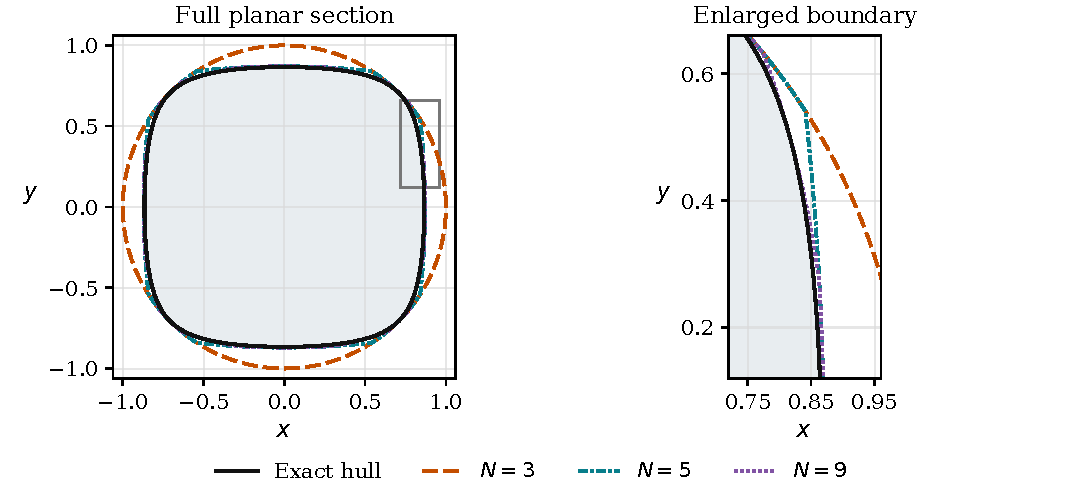
\includegraphics[width=\textwidth]{figures/finite-aggregation-slice.pdf}
 \caption{Sections by the plane $u=xe_1$, $v=ye_2$. The exact closed
 hull (black) is $(1-x^2)(1-y^2)\geq1/4$ inside $[-1,1]^2$.
 Colored curves bound the outer approximations from $N=3,5,9$ equally
 spaced angles in Lemma~\ref{lem:angle-mesh}; the right panel enlarges
 part of the first quadrant. The same planar sections occur for every
 $r\geq2$. The curves are computed from explicit radial formulas and
 illustrate the approximations; they are not estimates of their full
 Hausdorff errors.}
 \label{fig:finite-aggregation}
\end{figure}

\subsection{A lower bound allowing interior multipliers}

\begin{proof}[Proof of the lower bound in Theorem~\ref{thm:approximation-rate}]
Fix $F\subset\mathcal K_r\setminus\{0\}$ with $|F|\leq N$, and put
\[
 \eta=\frac1{400N^2},\qquad \epsilon=1/10.
\]
Use the $N+1$ parameters $\tau_j=1+j/N$, $j=0,\ldots,N$.
For each such $\tau$, choose $x_{\tau,\eta}=(u_{\tau,\eta},v_{\tau,\eta})$
with Gram matrix
\begin{equation}\label{eq:accuracy-gram}
 G_{\tau,\eta}=
 \begin{pmatrix}1-\epsilon/\tau&2/5-\eta\\
                 2/5-\eta&1-\epsilon\tau\end{pmatrix}.
\end{equation}
Here $0<\eta<1/10$, both diagonal entries are at least $4/5$,
and the off-diagonal entry has absolute value at most $2/5$.
Thus $\det G_{\tau,\eta}\geq12/25>0$. Such vectors exist in
$\R^2$ and embed in $\R^r$, with both norms at most one. They satisfy
\begin{equation}\label{eq:accuracy-values}
 f(x_{\tau,\eta})=(-\epsilon/\tau,-\epsilon\tau,\epsilon+\eta).
\end{equation}

Consider any $\lambda\in F$. If either $\lambda_1$ or $\lambda_2$
vanishes, goodness forces $\lambda_3=0$, and the nonzero cut is
strictly satisfied at every witness. Otherwise put
$t=\sqrt{\lambda_1/\lambda_2}>0$ and
$b=\sqrt{\lambda_1\lambda_2}$. If the cut excludes a witness,
then~\eqref{eq:accuracy-values} gives
\[
 \epsilon(\lambda_1/\tau+\lambda_2\tau-\lambda_3)
 <\eta\lambda_3.
\]
Using $\lambda_3\leq2b$ on both sides and dividing by
$\epsilon b$ yields $t/\tau+\tau/t<2a$, where $a=1+10\eta$.
If the same cut excludes a second parameter $\sigma$, adding the
two inequalities and applying the arithmetic--geometric mean
inequality gives
\[
 4a>(\tau+\sigma)\left(\frac{t}{\tau\sigma}+\frac1t\right)
 \geq\frac{2(\tau+\sigma)}{\sqrt{\tau\sigma}}.
\]
It follows that
\begin{equation}\label{eq:grid-exclusion}
 (\tau-\sigma)^2<4\tau\sigma(a^2-1)
 \leq16(a^2-1)
 =\frac4{5N^2}+\frac1{100N^4}<\frac1{N^2}.
\end{equation}
Distinct grid parameters differ by at least $1/N$. Thus one cut
excludes at most one of the $N+1$ witnesses. At most $N$ cuts
leave some $x_{\tau,\eta}$ in $P_F$. This finite pigeonhole
argument imposes no restriction on $t$ or extremality of $\lambda$.

For this witness the good multiplier
$\lambda_*=(\tau,1/\tau,2)$ has
$f_{\lambda_*}(x_{\tau,\eta})=2\eta>0$. Its leading matrix is
\[
 \begin{pmatrix}\tau&-1\\-1&1/\tau\end{pmatrix}\otimes I_r,
\]
which is positive semidefinite with operator norm
$\tau+1/\tau\leq5/2$. Hence
$\|\nabla f_{\lambda_*}(x)\|\leq5\sqrt2$ on the convex product
of the two unit balls. Both the witness and every $y\in D_r$
lie in that product, and $f_{\lambda_*}(y)\leq0$. The mean-value
inequality therefore gives
\[
 2\eta\leq f_{\lambda_*}(x_{\tau,\eta})-f_{\lambda_*}(y)
 \leq5\sqrt2\|x_{\tau,\eta}-y\|.
\]
Consequently
$d_H(D_r,P_F)\geq\sqrt2\eta/5$, proving the stated lower bound.
For an unbounded relaxation the bound holds with infinite left side.
\end{proof}

\subsection{Uniform objective gaps and an exact cut for one objective}

For a compact convex set $L$, write
$h_L(c)=\max_{x\in L}c\transpose x$. If $P_F$ is bounded, then
\begin{equation}\label{eq:hausdorff-support}
 d_H(D_r,P_F)=\sup_{\|c\|=1}\bigl(h_{P_F}(c)-h_{D_r}(c)\bigr).
\end{equation}
Indeed, choosing a closest point in $D_r$ bounds each support gap
above by the Hausdorff distance. Conversely, for $x\in P_F\setminus
D_r$ and its projection $y$ onto $D_r$, the unit vector
$c=(x-y)/\|x-y\|$ satisfies $h_{D_r}(c)=c\transpose y$ and
$h_{P_F}(c)\geq c\transpose x$. Taking the supremum gives the
reverse inequality; the case $P_F=D_r$ is immediate.

Thus Theorem~\ref{thm:approximation-rate} quantifies the worst gap
over unit linear objectives for one common bounded relaxation.
It applies to the final family even if the cuts were selected adaptively.
It does not give an iteration lower bound for solving one prescribed
objective. The next proposition makes that distinction explicit.

\begin{proposition}\label{prop:one-objective}
For every nonzero $c\in\R^{2r}$, there is a nonzero good multiplier
$\lambda\in\mathcal K_r$ such that
\begin{equation}\label{eq:one-objective}
 \min_{x\in D_r}c\transpose x
 =\min\{c\transpose x:f_\lambda(x)\leq0\}.
\end{equation}
Both minima are attained at a common point.
\end{proposition}
\begin{proof}
Let $F(x)=(f_1(x),f_2(x),f_3(x))$ and
$\mathcal K_r^*=\{z:\lambda\transpose z\geq0\text{ for all }
\lambda\in\mathcal K_r\}$. Convexity of every $f_\lambda$ for
$\lambda\in\mathcal K_r$ implies
\[
 \theta F(x)+(1-\theta)F(y)-F(\theta x+(1-\theta)y)
 \in\mathcal K_r^*\qquad(0\leq\theta\leq1).
\]
It follows directly that
\[
 E=\{(F(x)+z,c\transpose x+t):x\in\R^{2r},\
                            z\in\mathcal K_r^*,\ t\geq0\}
\]
is convex. It has nonempty interior because
$\mathcal K_r^*$ contains $\R^3_+$, and $t$ may increase freely.
The closed good-aggregation description of $D_r$ says that
$x\in D_r$ exactly when $-F(x)\in\mathcal K_r^*$.
Let $v=\min_{D_r}c\transpose x$ and choose a minimizer $x_*$,
which exists by compactness. Then $(0,v)\in E$, whereas
$(0,v-\delta)\notin E$ for every $\delta>0$.
Thus $(0,v)$ is a boundary point. A supporting hyperplane gives
a nonzero pair $(\lambda,\mu)$ satisfying
\[
 \lambda\transpose(F(x)+z)+\mu(c\transpose x+t)\geq\mu v
 \qquad(x\in\R^{2r},\ z\in\mathcal K_r^*,\ t\geq0).
\]
This supporting-hyperplane assertion does not require $E$ to be
closed: its nonempty interior has the same interior as its closure,
so one may support that closure at the included boundary point.
The recession directions $z,t$ and the bipolar theorem force
$\lambda\in\mathcal K_r$ and $\mu\geq0$.

For every nonzero $\lambda\in\mathcal K_r$,
\[
 f_\lambda(0)=-\lambda_1-\lambda_2+\lambda_3/2
 \leq-(\lambda_1+\lambda_2)/2<0.
\]
Evaluation at zero therefore rules out $\mu=0$. Normalize
$\mu=1$ to obtain
$f_\lambda(x)+c\transpose x\geq v$ for all $x$.
Evaluation at $x_*$, where $f_\lambda(x_*)\leq0$, gives
$f_\lambda(x_*)=0$. Also $\lambda\ne0$, since otherwise a
nonzero linear function would be bounded below on all of $\R^{2r}$.
For every $x$ satisfying $f_\lambda(x)\leq0$ we now have
$c\transpose x\geq v-f_\lambda(x)\geq v$, while $x_*$ attains
equality. Proposition~\ref{prop:ball-good-cone} ensures goodness.
\end{proof}

This is the usual strict-feasibility argument for conic convex duality,
specialized to the cone of convex aggregations; see
\citet[Section~5.9]{BoydVandenberghe2004}. The strict point is the
origin for the convex hull description, not for the original three
inequalities. Finding the objective-dependent multiplier can itself
require solving the original convex problem, and the proposition gives
no bound on that cost.

\subsection{Comparison with approximation theory}

The exponent two is familiar in convex approximation.
\citet{Rote1992} proves optimal $O(N^{-2})$ error bounds for
piecewise linear upper and lower approximations of univariate convex
functions on compact intervals with finite endpoint slopes, using
function values and supporting slopes, and treats
planar convex figures as well. This is particularly close context for
sampling a one-dimensional parameter family. His tangent-and-chord
approximations are different from the prescribed quadratic sublevel
sets considered here. The classical
polyhedral bounds of \citet{BronshteynIvanov1975}, and the modern
area-sensitive bounds and comparison in \citet[Section~1 and
Theorems~1--2]{AryaFonsecaMount2025}, concern approximation by vertices,
linear halfspaces, or piecewise affine functions. They provide the
appropriate context for quadratic local error from sampling a
one-dimensional family; they do not directly give
Theorem~\ref{thm:approximation-rate} for this prescribed cone of
quadratic cuts in $2r$ dimensions.

What is specific here is a two-sided bound for the HHC example, with a
lower bound against arbitrary interior good multipliers, constants
uniform in the replication dimension, and an exact rational
construction. It measures the size of a finite family of good
aggregations as an alternative to the exact finite SDP lift in
Theorem~\ref{thm:ball-hulls}. We assert no new general approximation
exponent, optimal constant, numerical conditioning guarantee, solver
improvement, or runtime lower bound.

\section{Four aggregations for three strict inequalities under PDLC}
\label{sec:four-aggregation}

The preceding example needs infinitely many good aggregations and does
not satisfy PDLC for its homogeneous matrices. We now establish the
sharp finite bound for three strict inequalities under that condition.
Here PDLC means that $Q_\theta\succ0$ for some $\theta\in\R^3$;
the coefficients of $\theta$ may have either sign.

\begin{theorem}[Four aggregations for strict PDLC systems]
\label{thm:strict-four}
Let $n\geq1$ and $m=3$. Suppose that $S\ne\varnothing$,
$\conv S\ne\R^n$, and $Q_1,Q_2,Q_3$ satisfy PDLC. Then there
are $1\leq\ell\leq4$ good multipliers $\lambda^1,\ldots,\lambda^\ell$
such that
\begin{equation}\label{eq:strict-four}
 \conv S=\bigcap_{j=1}^{\ell}\{x:f_{\lambda^j}(x)<0\}.
\end{equation}
Each $Q_{\lambda^j}$ has exactly one negative eigenvalue.
The original matrices need not be linearly independent, and the original
nonstrict feasible set need not be bounded or the closure of its interior.
For every $n\geq3$, four is necessary in some systems.
\end{theorem}

Blekherman and Dunbar's four-bound for regular nonstrict systems
\citep[Theorem~1.4]{BD2025,BDpreprint} is the substantive external
input. We transfer that bound to arbitrary strict systems by compact
inward perturbation and a limit that preserves strict validity.
Blekherman, Dey, and Sun previously gave an upper bound of six
\citep[Corollary~2.20]{BDSpreprint}; their Example~2.21 supplies the
sharpness construction below. Thus Theorem~\ref{thm:strict-four}
rules out the six-necessary example proposed in their Conjecture~3.2.
The number four and its lower-bound example are established antecedents;
the extension here concerns the unrestricted strict setting.

Dunbar's dissertation also states a four-bound for regular nonstrict
sets without the no-points-at-infinity hypothesis
\citep[Theorem~5.0.5]{Dunbar2025Thesis}. We acknowledge that stronger
prior statement and use only the fully qualified published theorem below.
To the best of our knowledge, the complete transfer to arbitrary strict
systems in Theorem~\ref{thm:strict-four} has not previously been given.
This claim concerns that transfer, including possible dependence of the
original matrices, rather than the first statement of a four-bound without
an infinity assumption. The negative-eigenvector limit used below has an
antecedent for a fixed feasible set in the proof of
\citet[Proposition~3.15, Section~8]{BDpreprint}.

\subsection{Regular inward perturbations}

We state the external input with its standing independence assumption.
For a triple $\widetilde Q_i$ with leading blocks $\widetilde A_i$,
the phrase \emph{no points at infinity} means
\begin{equation}\label{eq:no-infinity}
 \{d\in\R^n:d\transpose\widetilde A_i d\leq0\text{ for all }i\}
 =\{0\}.
\end{equation}

\begin{theorem}[Blekherman--Dunbar, external input]
\label{thm:bd-four-input}
Let $\widetilde Q_1,\widetilde Q_2,\widetilde Q_3\in\Sym^{n+1}$
be linearly independent and satisfy PDLC, and set
$C=\{x:(x,1)\transpose\widetilde Q_i(x,1)\leq0\text{ for all }i\}$.
If $\interior C\ne\varnothing$, $C=\cl(\interior C)$, and
\eqref{eq:no-infinity} holds, then
\[
 \cl(\conv C)=\bigcap_{j=1}^{\ell}
 \left\{x:(x,1)\transpose\Bigl(\sum_i\mu_i^j\widetilde Q_i\Bigr)(x,1)
 \leq0\right\}
 \qquad(\ell\leq4),
\]
where each $\mu^j\geq0$ is nonzero and each aggregated matrix has
at most one negative eigenvalue.
\end{theorem}

This is \citet[Theorem~1.4]{BD2025,BDpreprint}; no smoothness
assumption on the spectral curve is needed. The proof in the cited
preprint explicitly includes $n=1,2$ in Proposition~8.7 and combines
Propositions~8.6, 8.7, and 8.10. Consequently the input applies in
every positive dimension used here.

\begin{lemma}[Regular sublevels]\label{lem:regular-levels}
Let $h:M\to\R$ be continuous on a space with a countable base.
For all but at most countably many $c\in\R$,
\[
 \{h\leq c\}=\cl_M\{h<c\}.
\]
\end{lemma}
\begin{proof}
Continuity gives the inclusion from right to left. If it is strict,
there is $z$ with $h(z)=c$ and an open neighborhood $U$ of $z$
containing no point where $h<c$. Choose a basic open set $B$ with
$z\in B\subseteq U$. Then $c=\inf_{y\in B}h(y)$. There are at
most countably many such real infima, one for each basic open set.
\end{proof}

\begin{lemma}[Compact inward systems]\label{lem:inward-pdlc}
Under the hypotheses of Theorem~\ref{thm:strict-four}, there are
positive definite matrices $R_1,R_2,R_3$ and a decreasing sequence
$\varepsilon_k\downarrow0$ such that, on defining
\begin{align*}
 Q_i^\varepsilon&=Q_i+\varepsilon R_i,
 &w_i(x)&=(x,1)\transpose R_i(x,1),\\
 S_\varepsilon&=\{x:f_i(x)+\varepsilon w_i(x)<0\ \forall i\},
 &C_\varepsilon&=\{x:f_i(x)+\varepsilon w_i(x)\leq0\ \forall i\},
\end{align*}
each selected triple satisfies every hypothesis of
Theorem~\ref{thm:bd-four-input}. Moreover, $C_{\varepsilon_k}$ is
compact, $C_{\varepsilon_k}=\cl S_{\varepsilon_k}$,
$S_{\varepsilon_k}\subseteq S$, and every fixed finite subset of $S$
is contained in $S_{\varepsilon_k}$ for all sufficiently large $k$.
\end{lemma}
\begin{proof}
Since $n+1\geq2$, take, with standard basis vectors $e_1,e_2$,
\[
 R_1=I,\qquad R_2=I+e_1e_1\transpose,\qquad
 R_3=I+(e_1+e_2)(e_1+e_2)\transpose.
\]
These are positive definite and linearly independent: in a vanishing
linear combination the $(1,2)$ entry first forces the coefficient of
$R_3$ to vanish, and the two diagonal entries then force the others to
vanish. Write $B_i\succ0$ for their leading $n\times n$ blocks.
Lemma~\ref{lem:negative-direction} excludes a nonzero $d$ satisfying
$d\transpose A_i d<0$ for every $i$. Therefore, for every
$\varepsilon>0$, the inequalities
$d\transpose(A_i+\varepsilon B_i)d\leq0$ for all $i$ force $d=0$.
Thus the perturbed system has no points at infinity.

It is also bounded. Otherwise there would be $x_j\in C_\varepsilon$
with $\|x_j\|\to\infty$. After taking a subsequence,
$x_j/\|x_j\|\to d$ with $\|d\|=1$. Divide each perturbed
inequality by $\|x_j\|^2$ and take limits to obtain the forbidden
nonpositive leading inequalities at $d$. Closedness now makes
$C_\varepsilon$ compact.

Fix $x^0\in S$ and a PDLC certificate $\theta$. For every sufficiently
small $\varepsilon>0$, $x^0\in S_\varepsilon$ and
$Q_\theta+\varepsilon\sum_i\theta_iR_i\succ0$, by strictness and
continuity. The perturbed matrices are independent except at finitely
many parameters. Indeed, choose three coordinates of $\Sym^{n+1}$
on which the coordinate matrix of the $R_i$ has nonzero determinant.
The corresponding determinant for the $Q_i+\varepsilon R_i$ is a
cubic polynomial whose leading coefficient is that nonzero determinant.
Its zeros form a finite set. This argument does not assume independence
of the original $Q_i$.

Because every $w_i$ is positive, the continuous function
\[
 h(x)=\max_{1\leq i\leq3}\frac{f_i(x)}{w_i(x)}
\]
satisfies $S_\varepsilon=\{h<-\varepsilon\}$ and
$C_\varepsilon=\{h\leq-\varepsilon\}$. Apply
Lemma~\ref{lem:regular-levels} and choose $\varepsilon_k\downarrow0$
so that $-\varepsilon_k$ avoids its countable exceptional levels and
$\varepsilon_k$ avoids the finite dependence set, with every parameter
small enough for strict feasibility and PDLC. Such a sequence exists
because every nonempty real interval is uncountable. Then
\[
 C_{\varepsilon_k}=\cl S_{\varepsilon_k}
   =\cl(\interior C_{\varepsilon_k}),\qquad
 \interior C_{\varepsilon_k}\ne\varnothing.
\]
The second equality follows from
$S_{\varepsilon_k}\subseteq\interior C_{\varepsilon_k}
\subseteq C_{\varepsilon_k}$ and closedness. Positivity of $w_i$
gives $S_\varepsilon\subseteq S$. Finally, finitely many strict
inequalities at finitely many points remain strict for all sufficiently
small $\varepsilon$, proving the last assertion.
\end{proof}

\subsection{Strictification and the multiplier limit}

Two details are essential: a redundant nonstrict quadratic can remove
interior points when made strict, and a limiting quadratic can lose strict
validity unless its negative component is controlled.

\begin{lemma}[Strictification]\label{lem:strictification}
Let $U\subset\R^n$ be nonempty and open with bounded hull. Suppose
\[
 \cl(\conv U)=\bigcap_{j=1}^q\{x:p_j(x)\leq0\},
\]
where the $p_j$ are quadratic polynomials. After deleting every $p_j$
that is globally nonpositive, at least one inequality remains and
\[
 \conv U=\bigcap_{j\text{ retained}}\{x:p_j(x)<0\}.
\]
\end{lemma}
\begin{proof}
Deleting such polynomials preserves the nonstrict intersection. Some
inequality remains because a nonempty bounded hull is not $\R^n$.
If a quadratic $p$ vanishes at an interior point $x$ of $\{p\leq0\}$,
then $x$ is a local maximum with value zero. Its gradient vanishes and
its Hessian is negative semidefinite. The exact quadratic Taylor formula
therefore gives $p\leq0$ everywhere. For every retained polynomial this
is impossible, so $\interior\{p_j\leq0\}=\{p_j<0\}$.
The interior of a finite intersection equals the intersection of its
interiors. Finally, the nonempty open convex set $\conv U$ equals the
interior of its closure, which proves the formula.
\end{proof}

For completeness, the relevant negative components have a direct conic
description. If a symmetric matrix $M$ has exactly one negative eigenvalue
$-a<0$, choose its unit eigenvector $v$ and put $P=M+avv\transpose$.
Then $P\succeq0$, $Pv=0$, and
\begin{equation}\label{eq:negative-components}
 \{z:z\transpose Mz<0\}
 =\{z:\|P^{1/2}z\|<\sqrt a\,v\transpose z\}
  \;\cup\;
  \{z:\|P^{1/2}z\|<-\sqrt a\,v\transpose z\}.
\end{equation}
Both sets are convex, disjoint, and nonempty. This formula also covers
singular $M$ and the case $P=0$. A connected subset of the negative
sublevel lies in one of the two sets.

\begin{proof}[Proof of Theorem~\ref{thm:strict-four}, upper bound]
Use the sequence from Lemma~\ref{lem:inward-pdlc} and abbreviate
$S_k=S_{\varepsilon_k}$, $C_k=C_{\varepsilon_k}$.
Because $C_k=\cl S_k$,
\[
 \cl(\conv C_k)=\cl(\conv S_k).
\]
Indeed, each closed convex set containing $S_k$ also contains $C_k$,
and the reverse inclusion follows from $S_k\subseteq C_k$.
Theorem~\ref{thm:bd-four-input} followed by
Lemma~\ref{lem:strictification} gives a description of $\conv S_k$
by between one and four strict aggregations of the perturbed inequalities.
Every retained aggregation is good for $S_k$ and has exactly one
negative homogeneous eigenvalue, since it is strictly negative at $x^0$.
Duplicate multipliers to obtain four indices and normalize each in
the simplex $\Delta_3=\{\lambda\geq0:\sum_i\lambda_i=1\}$.
Write them as $\lambda^{k,j}$, $1\leq j\leq4$. By compactness,
after a common subsequence
$\lambda^{k,j}\to\lambda^j\in\Delta_3$ for every $j$.
Their matrices satisfy
\begin{equation}\label{eq:four-matrix-limit}
 M_{k,j}=Q_{\lambda^{k,j}}
       +\varepsilon_k\sum_i\lambda_i^{k,j}R_i
 \ \longrightarrow\ M_j=Q_{\lambda^j}.
\end{equation}
The perturbation term tends to zero because its norm is at most
$\varepsilon_k\max_i\|R_i\|$. Continuity of ordered eigenvalues
shows that $M_j$ has at most one negative eigenvalue. It has at least
one, since $f_{\lambda^j}(x^0)<0$. In particular every limiting
multiplier is nonzero and every limiting matrix has exactly one negative
eigenvalue.

Choose a unit negative eigenvector $v_{k,j}$ of $M_{k,j}$, oriented
so that $v_{k,j}\transpose(x^0,1)>0$. This scalar product cannot
vanish because the quadratic value at $(x^0,1)$ is negative. Take a
further common subsequence so that $v_{k,j}\to v_j$ for all $j$.
The unique negative eigenvalues converge to the negative eigenvalue of
$M_j$; passing to the eigenvector equation shows that $v_j$ is its
unit eigenvector.

Fix any $x\in S$. For all sufficiently large $k$, both $x$ and $x^0$
belong to $S_k$. The segment joining their lifts is strictly negative
for $M_{k,j}$, because the $k$th aggregation is good on $\conv S_k$.
The two scalar products with $v_{k,j}$ therefore have the same sign:
otherwise that segment would meet $v_{k,j}^{\perp}$, where $M_{k,j}$
is positive semidefinite. Hence $v_{k,j}\transpose(x,1)>0$.
Taking limits gives $v_j\transpose(x,1)\geq0$. Equality is
impossible, since $f_{\lambda^j}(x)<0$ and $M_j$ is positive
semidefinite on $v_j^\perp$. Thus every lift of every point of $S$
lies in the same convex negative component of $M_j$ in
\eqref{eq:negative-components}. All finite convex combinations of these
lifts remain in that component. This proves
\[
 \conv S\subseteq\bigcap_{j=1}^4\{x:f_{\lambda^j}(x)<0\}
\]
and proves strict goodness of every limit.

Conversely, a point strictly satisfying all four limiting inequalities
strictly satisfies all four perturbed inequalities for sufficiently
large $k$, by \eqref{eq:four-matrix-limit} and finiteness of the
index set. It then belongs to $\conv S_k\subseteq\conv S$.
This proves \eqref{eq:strict-four}; remove repeated multipliers if
desired. No closure is taken in this last argument.
\end{proof}

\begin{remark}[Dependent triples]\label{rem:dependent-four}
The preceding proof already covers dependence. A stronger bound of two
follows from the classical two-constraint result and the cone reduction
also noted in \citet[Section~2.5, after Example~2.21]{BDSpreprint}.
Indeed, evaluation at
a fixed feasible lift is strictly negative on every nonzero nonnegative
combination of the $Q_i$. Their finitely generated cone is therefore
pointed. If their span has dimension at most two, intersecting this cone
with the affine hyperplane on which that evaluation is $-1$ gives a
compact segment or a point. Its at most two endpoints lie on rays
generated by original matrices. Every original inequality is a nonzero
nonnegative combination of those at most two inequalities, so they define
the same $S$. Applying \citet[Theorem~1]{Yildiran2009}, with its
opposite sign convention, gives at most two good aggregations; translating
their multipliers back to the original rows preserves goodness. A single
remaining inequality may be duplicated when applying that theorem.
This observation is not needed for the four-bound.
\end{remark}

\subsection{Sharpness and the closed hull}

\begin{example}[The four-necessary example of Blekherman--Dey--Sun]
\label{ex:four-sharp}
Let $n\geq3$, $s=x_1$, and $\rho=\sum_{i=2}^n x_i^2$. Consider
\begin{equation}\label{eq:four-sharp-system}
 f_1=-s^2+1+\rho,\qquad
 f_2=s^2+5s-4+\rho,\qquad f_3=-s-\rho.
\end{equation}
This is \citet[Example~2.21]{BDSpreprint}. The identity
$-7f_1-3f_2-15f_3=4s^2+5\rho+5$ proves PDLC.
The point $(s,\rho)=(-3,4)$ is strictly feasible. Every feasible point
has $s<-1$: $f_1<0$ forces $|s|>1$, while $f_2<0$ excludes $s>1$.
Consequently the hull is proper, and the $f_1$ inequality is good because
these points lie in its negative $s$ component. The convex ball inequality
$f_2<0$ is good as well. The two sums are
\[
 f_1+f_3=-s^2-s+1,
 \qquad f_2+f_3=s^2+4s-4.
\]
The first has one negative homogeneous eigenvalue and is negative on
the interval $s<\alpha=(-1-\sqrt5)/2$ containing every feasible $s$.
The second is convex and also has one negative homogeneous eigenvalue.
Thus the following four rays are good:
\[
 r_1=(1,0,0),\quad r_2=(0,1,0),\quad
 r_3=(1,0,1),\quad r_4=(0,1,1).
\]

We verify directly that each ray is indispensable. If $(a,b,c)$ is good,
then $c\leq a+b$: otherwise the coefficient $a+b-c$ of $\rho$ gives
at least $n-1\geq2$ negative eigenvalues. Hence every good multiplier
belongs to
\begin{equation}\label{eq:four-ray-cone}
 \{(a,b,c)\geq0:c\leq a+b\}=\cone\{r_1,r_2,r_3,r_4\}.
\end{equation}
For the equality, choose $t\in[\max(0,c-b),\min(a,c)]$ and write
$(a,b,c)=(a-t)r_1+(b-c+t)r_2+tr_3+(c-t)r_4$.
Put $\beta=-2-2\sqrt2$. The four witnesses below have the displayed
slacks in the order $(f_{r_1},f_{r_2},f_{r_3},f_{r_4})$:
\[
\begin{array}{c|c|c}
 \text{designated ray}&(s,\rho)&\text{slacks}\\\hline
 r_1&(-2,3)&(0,-7,-1,-8)\\
 r_2&(-4,8)&(-7,0,-11,-4)\\
 r_3&(\alpha,0)&(\alpha,4\alpha-3,0,3\alpha-3)\\
 r_4&(\beta,0)&(4\beta-3,\beta,3\beta-3,0).
\end{array}
\]
Every off-designated slack is strictly negative, since $\alpha,\beta<0$.
Each witness is realizable by setting $x_2=\sqrt\rho$ and the other
coordinates to zero. At the witness for $r_j$, any nonzero multiplier in
\eqref{eq:four-ray-cone} is strictly negative unless it is a positive
multiple of $r_j$. But that witness is outside $\conv S$, since its
designated good inequality is zero. Every exact strict-good description
must therefore contain all four rays. The upper bound already proved
then implies that these four inequalities describe the hull exactly.
This proves the sharpness assertion in Theorem~\ref{thm:strict-four}.
The argument makes no sharpness claim for $n=1,2$.
\end{example}

The strict result also provides a closed conic description, provided the
negative components retain their orientation. The conic representation
principle is already recorded in \citet[Remark~2.19]{BDSpreprint};
the bound of four follows
from Theorem~\ref{thm:strict-four}.

\begin{corollary}[Four oriented second-order cone constraints]
\label{cor:four-soc}
Under the hypotheses of Theorem~\ref{thm:strict-four}, choose its
multipliers and write $Q_{\lambda^j}=P_j-v_jv_j\transpose$ with
$P_j\succeq0$, $P_jv_j=0$, and
$v_j\transpose(x^0,1)>0$ for one $x^0\in S$. Then
\begin{align}
 \conv S&=\{x:\|P_j^{1/2}(x,1)\|<v_j\transpose(x,1)
                    \text{ for }1\leq j\leq\ell\},\label{eq:four-soc-open}\\
 \cl(\conv S)&=\{x:\|P_j^{1/2}(x,1)\|\leq v_j\transpose(x,1)
                    \text{ for }1\leq j\leq\ell\}.\label{eq:four-soc-closed}
\end{align}
\end{corollary}
\begin{proof}
Use the spectral decomposition in \eqref{eq:negative-components},
absorbing the square root of the negative eigenvalue's magnitude into
$v_j$. Strict goodness and connectedness place $\conv S$ in the
component containing $(x^0,1)$. The intersection of those components
contains the hull and is contained in \eqref{eq:strict-four}, proving
\eqref{eq:four-soc-open}. Its closed version contains the closure.
Conversely, let $x$ satisfy every closed conic inequality and put
$x_t=(1-t)x+tx^0$, $0<t\leq1$. Convexity of the norm gives
\[
 v_j\transpose(x_t,1)-\|P_j^{1/2}(x_t,1)\|
 \geq t\bigl(v_j\transpose(x^0,1)-\|P_j^{1/2}(x^0,1)\|\bigr)>0.
\]
Thus $x_t\in\conv S$ and $x_t\to x$ as $t\downarrow0$.
\end{proof}

Replacing $<$ by $\leq$ in \eqref{eq:strict-four} without keeping
the orientations need not give this closure. Nor must this closure
equal the hull of the original nonstrict set. For example, for $n\geq2$,
take the half-ball example of \citet[Example~2.23]{BDSpreprint} and
append one redundant inequality:
\[
 f_1=-x_1^2+x_1,\qquad f_2=\|x\|^2-1,\qquad
 f_3=-\|x\|^2-1.
\]
Here $-Q_3=I$, so PDLC holds, and
$S=\conv S=\{x:x_1<0,\ \|x\|<1\}$. The first two strict
inequalities are good and describe $S$. Their nonstrict counterparts
describe the closed half-ball together with the isolated point $e_1$.
The original nonstrict set contains that same extra point. Its hull is
therefore larger than $\cl(\conv S)$.

Theorem~\ref{thm:strict-four} is an existence result for a fixed finite
description. Its proof does not supply an efficient multiplier-selection
algorithm or coefficient-size bounds. The exact checks accompanying this
section verify the finite identities and witnesses in
Example~\ref{ex:four-sharp}; the perturbation and limiting arguments are
proved above rather than inferred from those checks.

\section{Formal verification and reproducible supplements}
\label{sec:formal-overview}

The accompanying Lean development verifies specified parts of the
paper. It has 64 modules with 909 owned declarations, plus five imported
local support modules. The portable sources, pinned Lean~4.33.1
toolchain and Mathlib dependency manifest, declaration coverage maps,
and a targeted verification runner are in \path{supplement/lean/}. A
separate formal supplement relates the theorem interfaces to the
mathematical statements. The table lists the five packages; sizes are
modules / owned declarations, and package numbers only label the
supplied audit partitions.

\begin{center}
\small
\begin{tabular}{@{}p{0.09\textwidth}p{0.12\textwidth}p{0.69\textwidth}@{}}
\hline
Package & Size & Verified mathematical scope\\
\hline
27 & 11 / 178 & Theorem~\ref{thm:certificate}, its HHC specialization,
AHC sequence equivalence, and the principal separation and cone lemmas.\\[3pt]
28 & 10 / 158 & Closed-hull properness, the unconditional whole-space Shor
criterion and its AHC consequences, exact signed-coordinate SDP tests,
Dines' theorem, Example~\ref{ex:strip}, and the strict-feasibility
counterexample of Example~\ref{ex:closed} ($S=\varnothing$, the form of
$T$, proper hull, trivial convex certificates, and HHC); its interior
and good-multiplier arguments are not formalized.\\[3pt]
29 & 18 / 248 & Actual HHC for $S_r$, $r\geq2$, the eigenvalue-based good
cone, indispensable uncountably many strict rays, and impossibility of a
finite weak good-aggregation description.\\[3pt]
30 & 10 / 93 & Exact hull and lift assertions of Theorem~\ref{thm:ball-hulls}: the two-point
construction in every $r\geq2$, exact strict and closed hulls, PD/PSD lifts,
weak-system hull equality, and all-good intersection formulas.\\[3pt]
31 & 15 / 232 & Explicit Euclidean approximation bounds, the
$\Theta(N^{-2})$ rate, tolerance families, and exact rational meshes with
logarithmic coefficient sizes.\\
\hline
\end{tabular}
\end{center}

Two formal statements differ from the paper. Package~28 checks
$n(n+1)+2n$ signed coordinate objectives; the shorter $2n+1$
trace-and-vector test of Corollary~\ref{cor:finite-sdp} is proved only
in the paper. Package~31 proves the upper bound of
Theorem~\ref{thm:approximation-rate} and the lower bound
$1/(2000N^2)$, which implies the weaker bound
$\sqrt2(\log2)^2/(1600N^2)$ stated in that package; the lower constant $\sqrt2/2000$ used
in this paper is not formalized. The formal approximation model
explicitly transports the Euclidean norm on all $2r$ coordinates rather
than using a product maximum norm.

The formal definitions use actual feasible sets, ordinary convex hulls,
nonnegative aggregation weights, and homogeneous eigenvalues. HHC of the
example is proved, not assumed; the exact-hull package proves its
two-point construction without a general HHC hull theorem as a premise;
and the certificate proof derives its separation weights and nonzero
coefficient limit. None of these enters the theorem interfaces as a
hidden assumption.

For each package, warning-free targeted compilation, a transitive axiom
audit of all owned declarations, and per-module kernel replay have passed
with recorded source fingerprints. The audit permits only
\texttt{propext}, \texttt{Classical.choice}, and \texttt{Quot.sound}.
The supplied runner reproduces these checks for the portable project and
records whether its inputs are unchanged. Kernel replay uses Lean's
kernel and the imported dependencies; it does not rebuild and replay all
dependencies, and it is not an independent proof-assistant
implementation. Exact rational checks of the examples and the
figure-generation program are also supplied; they check stated
identities and witnesses, not universal theorems.

The Lean verification does not cover, among others, the general sharp
Gram-map theorem,
the arbitrary-quadratic obstruction, countable dense weak sufficiency,
the four-aggregation PDLC theorem,
the many-row appendix, the local-certificate application, the
single-objective duality result, the sufficient criteria of
Proposition~\ref{prop:stable}, the general closure equality of
Proposition~\ref{prop:shor-closure}, or
Examples~\ref{ex:nonclosed-shor}, \ref{ex:ahc-not-hhc},
\ref{ex:hhc-not-stable}, and~\ref{ex:ordinary-hc}. The spectral quantitative alternative
to the certificate proof is not fully formalized. Literature priority
and numerical solver correctness are outside every package. For these
results the paper supplies the mathematical proofs and source
comparisons.

\section{Discussion}
\label{sec:discussion}

The results distinguish three kinds of information obtainable from
quadratic aggregation. Under asymptotic hyperplane convexity, a single
nonconstant globally convex aggregation detects whether a nonempty
strict system has a proper hull. Complete hull descriptions require a
larger class of good aggregations. Their size depends on geometry that
the certificate alone does not record: homogeneous PDLC for three rows
gives a sharp four-bound, whereas HHC without that definiteness can require
uncountably many strict quadratic inequalities even in four variables.
The latter example still has a small exact semidefinite lift and
quantitatively controlled finite approximations.

Several distinctions persist at the boundaries of these results.
Strict feasibility supports the certificate theorem and the comparison
with the Shor projection; closed systems without a strictly feasible
point need separate treatment. Closure also changes representation
cardinality: the explicit open hull needs uncountably many strict
quadratics, while a countable dense good family suffices for its closed
hull. Under PDLC the limiting negative components must retain their
orientation to obtain a valid closed conic description. None of these
operations can be replaced in general by changing inequality signs.

The statements are structural rather than complexity guarantees.
No general procedure for recognizing HHC or for efficiently selecting the
four PDLC multipliers is established here. The exact SDP characterizations
use exact optimal values, and the rational approximation families control
coefficient size without analyzing numerical conditioning. For a
three-dimensional span with many extreme rays, the directional facet
bound improves the known count under its stated cone condition; the
counterexample in Appendix~\ref{app:three-span} rules out a general
constant bound from the complementary condition alone. These limits
define the reach of the proved results without being premises on which
any theorem in the paper remains contingent.

\appendix
\section{An elementary application to local infeasibility certificates}
\label{app:application}

Convex aggregation can turn a local affine proof into a globally valid
convex inequality. We give the exact certificate and a small example.
Both apply established aggregation and convexification principles; we
make no claim of algorithmic novelty or performance. In related
conflict analysis,
\citet{BertholdWitzig2021} use local affine proofs and aggregate
convex nonlinear relaxation rows. \citet{Dong2016} explicitly
allows aggregation of original quadratic inequalities or quadratic
rows reconstructed from a lift before convexification. The
construction below selects nonnegative weights for the original
quadratic rows while retaining an affine box margin.

\subsection{Validity and a linear selection problem}

Let $f_i(x)\leq0$ be globally active quadratic rows as in
\eqref{eq:system}. On a nonempty bounded box $B=[l,u]$, suppose
the affine functions
$\ell_i(x)=a_i\transpose x+d_i$ satisfy
$\ell_i(x)\leq f_i(x)$ for all $x\in B$.
For $\lambda\geq0$, put
$L_\lambda=\sum_i\lambda_i\ell_i$.

\begin{proposition}\label{prop:local-certificate}
If $\min_{x\in B}L_\lambda(x)\geq\delta>0$, the box $B$
contains no point satisfying all the original rows. If also
$A_\lambda\succeq0$, then, for every $\bar x\in\R^n$,
\begin{equation}\label{eq:global-tangent}
 f_\lambda(\bar x)+\nabla f_\lambda(\bar x)\transpose(x-\bar x)
 \leq0
\end{equation}
is valid for every original feasible point. It separates every
expansion point $\bar x\in B$. If $\bar x$ minimizes
$f_\lambda$ on $B$, this one tangent excludes the entire box.
\end{proposition}
\begin{proof}
Original feasibility implies $f_\lambda\leq0$ everywhere on the
feasible set, whereas on $B$ the estimator inequality gives
$f_\lambda\geq L_\lambda\geq\delta>0$.
For a convex quadratic, subtraction of its tangent at $\bar x$
leaves $(x-\bar x)\transpose A_\lambda(x-\bar x)\geq0$.
This proves global validity and separation at any $\bar x\in B$.
A minimizer on the compact box exists, and the convex first-order
condition gives
$\nabla f_\lambda(\bar x)\transpose(x-\bar x)\geq0$ for
all $x\in B$. Its tangent is therefore at least $\delta$ throughout
the box.
\end{proof}

An arbitrary tangent separates its expansion point but need not
exclude all of $B$. The quadratic aggregate remains globally valid
even though the estimators used to select its weights are local.
When several estimators refer to the same original row, their
weights must be summed in reconstructing that row's coefficient.

A sufficient positive-semidefiniteness condition is symmetric
diagonal dominance with nonnegative diagonal. Let
$a(\lambda)=\sum_i\lambda_i a_i$ and
$d(\lambda)=\sum_i\lambda_i d_i$. Consider the linear program
\begin{equation}\label{eq:repair-lp}
\begin{aligned}
 \max_{\lambda,t,v,\delta}\quad&\delta\\
 \text{subject to}\quad
 &\lambda\geq0,\qquad\sum_i\lambda_i=1,\\
 &t_{jk}\geq (A_\lambda)_{jk},\quad
  t_{jk}\geq-(A_\lambda)_{jk} &&(j<k),\\
 &(A_\lambda)_{jj}\geq\sum_{k<j}t_{kj}+\sum_{k>j}t_{jk}
                                                    &&(j=1,\ldots,n),\\
 &v_j\leq0,\quad v_j\leq a_j(\lambda) &&(j=1,\ldots,n),\\
 &\delta\leq d(\lambda)+l\transpose a(\lambda)
                         +\sum_j(u_j-l_j)v_j.
\end{aligned}
\end{equation}
The last expression is a lower bound on the exact affine minimum
\begin{equation}\label{eq:box-minimum}
 \min_{x\in B}L_\lambda(x)
 =d(\lambda)+l\transpose a(\lambda)
                    +\sum_j(u_j-l_j)\min\{0,a_j(\lambda)\}.
\end{equation}
It attains that minimum by choosing
$v_j=\min\{0,a_j(\lambda)\}$. Likewise the absolute-value lifts
can be chosen as $t_{jk}=|(A_\lambda)_{jk}|$.
Thus~\eqref{eq:repair-lp} optimizes exactly the affine margin over
the normalized diagonally dominant aggregates. Any feasible solution
with certified $\delta>0$ suffices for validity; no optimality
certificate is needed. The elementary identity
\begin{equation}\label{eq:dd-sos}
 x\transpose A x=
 \sum_j\left(A_{jj}-\sum_{k\ne j}|A_{jk}|\right)x_j^2
 +\sum_{j<k}|A_{jk}|
             (x_j+\operatorname{sign}(A_{jk})x_k)^2
\end{equation}
proves positive semidefiniteness whenever the diagonal dominance
conditions hold. Zero off-diagonal terms may be omitted. For rational
data and rational weights, all coefficients and the margin can be
checked exactly. Diagonal dominance is sufficient, not necessary,
and depends on the chosen coordinates.

Affine equalities $h_e(x)=0$ may be included with signed weights
$\mu_e$. Add $\sum_e\mu_e h_e$ to both the original aggregate and
its affine estimator. To normalize the selection problem, write
$\mu_e=\mu_e^+-\mu_e^-$, with nonnegative parts, and replace the
simplex equation by
\[
 \sum_i\lambda_i+\sum_e(\mu_e^++\mu_e^-)=1.
\]
This permits equality-only certificates and bounds every multiplier.
Normalizing only the inequality weights is insufficient: with the
row $-1\leq0$, equality $x=0$, and $B=[1,2]$, the aggregate
$-1+\mu x$ has margin $\mu-1$ for $\mu\geq0$. Its margin is
unbounded if $\mu$ is left unnormalized, although each individual
certificate is valid. The equality extension is for affine
equalities, whose signed affine estimators are exact.

If original rows are imposed only when specified logical conditions
are active, their aggregate is valid under the conjunction of the
conditions supporting its nonzero weights. This condition must be
retained in any resulting cut. Global unconditional validity in
Proposition~\ref{prop:local-certificate} uses globally active rows.

\subsection{A complete rational example}

Let $0\leq x,y\leq1$ and impose
\begin{equation}\label{eq:repair-example}
 f_1=x^2+2xy-\frac3{50}\leq0,
 \qquad
 f_2=2y^2-xy-\frac9{100}\leq0.
\end{equation}
The two quadratic matrices have determinants $-1$ and $-1/4$,
so both are indefinite. The relaxation with square variables
$s_x,s_y$ and product variable $w$ imposes the full square envelopes
and the four McCormick inequalities,
\[
 x^2\leq s_x\leq x,\qquad y^2\leq s_y\leq y,
 \qquad\max\{0,x+y-1\}\leq w\leq\min\{x,y\},
\]
along with $s_x+2w\leq3/50$ and $2s_y-w\leq9/100$.
It admits $(x,y,s_x,s_y,w)=(1/5,1/5,1/25,1/25,0)$.
This is the complete termwise convex relaxation on the root box;
the failure is not due to missing square tangents.

On the smaller box $B=[1/5,1]^2$, take
\[
 \ell_1=\frac45x+\frac25y-\frac9{50},\qquad
 \ell_2=-x+\frac35y+\frac3{100}.
\]
Their validity follows from the polynomial identities
\[
 \begin{split}
 f_1-\ell_1&=(x-1/5)^2+2(x-1/5)(y-1/5),\\
 f_2-\ell_2&=2(y-1/5)^2+(1-y)(x-1/5),
 \end{split}
\]
whose right sides are nonnegative on $B$. We have
\[
 2\ell_1+\ell_2=\frac35x+\frac75y-\frac{33}{100}
                         \geq\frac7{100}>0.
\]
The original aggregate is
\[
 G=2f_1+f_2=2x^2+3xy+2y^2-\frac{21}{100}
   =\frac12x^2+\frac12y^2+\frac32(x+y)^2-\frac{21}{100}.
\]
Its quadratic matrix is positive definite, with determinant $7/4$.
At $\bar x=\bar y=1/5$, the value of $G$ is $7/100$ and its
gradient is $(7/5,7/5)$. Its tangent inequality is exactly
\begin{equation}\label{eq:repair-tangent}
 x+y\leq\frac7{20}.
\end{equation}
It excludes the root relaxation witness and the entire smaller box,
where $x+y\geq2/5>7/20$.

The origin and $(1/5,0),(0,1/5)$ satisfy both original rows, so the
system is globally feasible. With binary variables $z_x,z_y$ and
the additional inequalities $x\geq z_x/5$, $y\geq z_y/5$, either
single activation is feasible but joint activation is infeasible.
Also $\min_B\ell_1=3/50>0$: a one-row local proof may use only
the first, indefinite row, whereas the displayed convex aggregate
uses both rows. No general support-selection guarantee follows.

For completeness the selection LP has an exact solution here.
Write $\lambda=(a,1-a)$, $0\leq a\leq1$. Its matrix is
\[
 A_\lambda=\begin{pmatrix}
 a&(3a-1)/2\\(3a-1)/2&2(1-a)
 \end{pmatrix}.
\]
The inequalities $a\geq|(3a-1)/2|$ and
$2(1-a)\geq|(3a-1)/2|$ reduce to
$1/5\leq a\leq5/7$.
The affine coefficients of $L_\lambda$ are
$(9a/5-1,\,3/5-a/5)$, and its constant is $(3-21a)/100$.
The second coefficient is positive, while the first changes sign
at $a=5/9$. Formula~\eqref{eq:box-minimum} gives
\[
 \min_B L_\lambda=
 \begin{cases}
 (31a-17)/20,&a\leq5/9,\\
 (11a-5)/100,&a\geq5/9.
 \end{cases}
\]
Both pieces are strictly increasing and agree at their common
endpoint. Thus the exact optimum is
$\lambda=(5/7,2/7)$ with normalized margin $1/35$.
The illustrative weights $(2,1)$ have normalized margin $7/300$;
their unnormalized margin $7/100$ is not comparable to $1/35$.

\subsection{Limits of this application}

If the quadratic rows are purely bilinear, their quadratic matrices
have zero diagonal. Any positive semidefinite aggregate then
vanishes: each $2\times2$ principal minor gives
$0\leq-A_{jk}^2$, hence $A_{jk}=0$ for every $j,k$.
Signed combinations of purely bilinear equalities have the same
obstruction. Cancellation can produce an affine aggregate but
cannot produce nonzero positive semidefinite curvature.

Finally every positive semidefinite aggregate is implied by the
common Shor lift, by~\eqref{eq:shor-aggregation}; its tangents are
implied as well. The example demonstrates strength beyond the
termwise relaxation, not beyond the full Shor relaxation. The
existence theorem does not guarantee a positive-margin diagonally
dominant solution on a prescribed local support. The validity
statements above do not depend on any solver implementation or
empirical result.

The accompanying script \texttt{supplement/check\_examples.py}
uses rational arithmetic to check the displayed polynomial
identities, margins, lifted witnesses, and selected matrix
calculations. These checks supplement the proofs and do not prove the
universal statements.

\section{Many constraints in a three-dimensional matrix span}
\label{app:three-span}

The number of generators matters when the homogeneous matrices span a
three-dimensional space but more than three constraints are present.
This appendix gives an elementary directional refinement of the known
facet bound and an obstruction to extending the two-aggregation case to
arbitrary polyhedral coefficient cones. These are supporting consequences
and examples, rather than a new topological aggregation theorem.

Let $n\geq3$, $L=\spanop\{Q_1,\ldots,Q_m\}$ have dimension three,
and suppose that $L$ contains a positive definite matrix. Assume
$S\ne\varnothing$ and $\conv S\ne\R^n$. Define the matrix cone
\[
 \mathcal C_L=\cone\{Q_1,\ldots,Q_m\}\subset L,
 \qquad \mathcal P_L=L\cap\Sym^{n+1}_+.
\]
We distinguish $\mathcal C_L$ from the multiplier cone $\mathcal K$
in \eqref{eq:certificate-cone}. For $M\in L$, write
$q_M(x)=(x,1)\transpose M(x,1)$.
Evaluation at a fixed feasible lift is negative on every nonzero
nonnegative combination of the generators. It follows that $\mathcal C_L$
is pointed. A section on which the negative of that evaluation equals one
is the convex hull of the normalized generators, hence is a compact
polygon. If $\mathcal C_L$ has $k$ extreme rays, it consequently has
$k$ facets, each generated by two extreme rays. We may retain one
original matrix on each extreme ray: every omitted row is a nonzero
nonnegative combination of the retained rows, so the strict set and the
available aggregation matrices are preserved.

Blekherman, Dey, and Sun give the resulting $2k$ bound
\citep[Proposition~2.22]{BDSpreprint}. Their proof uses the facets of
this three-dimensional cone. The next proposition records how the count
depends on the chosen positive definite direction; its three-generator
antecedent is \citet[Proposition~8.6]{BDpreprint}.

\begin{proposition}[Directional facet bound]\label{prop:facet-bound}
Write an irredundant facet representation
\[
 \mathcal C_L=\{M\in L:\ell_j(M)\geq0,\ j=1,\ldots,k\}.
\]
For every $D\in L$ with $D\succ0$, put
$J_-(D)=\{j:\ell_j(D)<0\}$. Then $\conv S$ is described by
at most $2|J_-(D)|$ good aggregations. In particular,
\begin{equation}\label{eq:conditional-facet-bound}
 \mathcal P_L\not\subseteq-\mathcal C_L
 \quad\Longrightarrow\quad
 \text{at most }2k-2\text{ good aggregations suffice}.
\end{equation}
\end{proposition}
\begin{proof}
First, the full system has HHC. Choose three basis matrices for $L$.
On each homogeneous hyperplane their restrictions still admit a positive
definite real combination. That hyperplane has dimension $n\geq3$, so
the three-form convexity theorem \citep[Theorem~2.1]{Polyak1998}
gives a convex joint image. The image of the original $m$ forms is a
linear image of this convex image. The full good-aggregation description
therefore applies \citep[Theorem~2.9]{BDSpreprint}.

Since $D\succ0$ has positive evaluation at a feasible lift, it cannot
belong to $\mathcal C_L$. Thus $J_-(D)$ is nonempty. Let $M\in\mathcal C_L$
be a good aggregation matrix whose strict sublevel is not all of
$\R^n$. It has exactly one negative eigenvalue. Set
\[
 t_* =\min_{j\in J_-(D)}
       \frac{\ell_j(M)}{-\ell_j(D)},\qquad M_*=M+t_*D.
\]
Every facet inequality remains satisfied up to $t_*$, and at least one
indexed by $J_-(D)$ becomes an equality. Hence $M_*\in\mathcal C_L$
lies on a selected facet. Also $M_*\ne0$: for $t_*=0$ this follows
from $M\ne0$, and for $t_*>0$ the alternative would make
$M=-t_*D$ negative definite, contrary to its inertia.

The positive semidefinite improvement lemma
\citep[Proposition~9.1]{BDSpreprint} shows that $M_*$ is good and
$\{q_{M_*}<0\}\subseteq\{q_M<0\}$. To check its coefficient
hypothesis, choose nonnegative representations $M=Q_\lambda$ and
$M_*=Q_\mu$. Then $Q_{\mu-\lambda}=t_*D\succeq0$ and
$\lambda+(\mu-\lambda)=\mu\geq0$, with $\mu\ne0$. Thus every
nonredundant good cut is dominated by a good cut on a selected facet.
The intersection of all good cuts on these facets equals the hull:
it contains the hull by goodness and is contained in every original good
cut by this domination.

On each facet the available matrices are nonnegative combinations of
its two extreme generators. The pair-support reduction
\citep[Proposition~9.6]{BDSpreprint} describes the intersection of its
good cuts using at most two such cuts. Goodness here is relative to the
full set $S$, as in that proposition, not to the two-row subsystem.
Facets without good cuts contribute no inequality. Summing over the
selected facets proves $2|J_-(D)|$.

Finally, if $E\in\mathcal P_L\setminus(-\mathcal C_L)$, some
$\ell_j(E)>0$. Choose $D_0\succ0$ in $L$. For sufficiently small
$\delta>0$, $D=E+\delta D_0\succ0$ and $\ell_j(D)>0$.
Thus $|J_-(D)|\leq k-1$, proving
\eqref{eq:conditional-facet-bound}.
\end{proof}

Minimizing $|J_-(D)|$ over positive definite $D\in L$ can strengthen
the displayed bound for a particular cone. This is an existence bound;
no procedure for finding a best direction or the endpoint multipliers is
asserted. The proof uses strict aggregation directly and requires no
regularity or boundedness assumption on the original weak feasible set.

\begin{example}[An arbitrarily large necessary family of ellipsoids]
\label{ex:many-ellipsoids}
Let $m\geq3$, $n\geq2$, and $0<a_1<\cdots<a_m<1$. Put
$\rho=\sum_{j=2}^n x_j^2$ and define
\begin{equation}\label{eq:many-ellipsoids}
 f_i(x)=a_i x_1^2+(1-a_i^2)\rho-1,\qquad
 U=\{x:f_i(x)<0\text{ for all }i\}.
\end{equation}
Then $U$ is nonempty, open, bounded, and convex, since its defining
quadratic parts are positive definite and the origin is strictly feasible.
In the basis $(x_1^2,\rho,t^2)$ of the homogeneous span, the matrices
have coordinate vectors $(a_i,1-a_i^2,-1)$. For $a<b<c$,
\begin{equation}\label{eq:span-vandermonde}
 \det\begin{pmatrix}a&1-a^2&-1\\b&1-b^2&-1\\c&1-c^2&-1\end{pmatrix}
 =(b-a)(c-a)(c-b)>0.
\end{equation}
This follows by the elementary column operations that turn the matrix
into a Vandermonde matrix. Hence the span is exactly three-dimensional
and contains the positive definite form $x_1^2+\rho+t^2$.

For each $i$, choose $p_i$ with
\begin{equation}\label{eq:many-witness}
 (p_i)_1^2=\frac{2a_i}{1+a_i^2},\qquad
 \sum_{j=2}^n(p_i)_j^2=\frac1{1+a_i^2}.
\end{equation}
For example, take the positive square roots in coordinates one and two
and zeros elsewhere. Direct substitution gives the identity
\begin{equation}\label{eq:many-witness-slack}
 f_j(p_i)=-\frac{(a_j-a_i)^2}{1+a_i^2}.
\end{equation}
Thus, at $p_i$, a nonzero nonnegative aggregation is nonnegative
exactly when its multiplier is a positive multiple of $e_i$.
Since $p_i\notin U=\conv U$, every exact strict aggregation family,
even an infinite one, must contain that ray. The original $m$ rows are
good, so the minimum finite cardinality is exactly $m$. Each row has
exactly one negative homogeneous eigenvalue. The witness also exposes
its matrix ray in $\mathcal C_L$: all other generators have strictly
negative evaluation at $p_i$. In particular $k=m$.

The same necessity holds for finite nonstrict aggregation descriptions
of $\cl U$. Indeed, if a finite family omits ray $i$, all its
inequalities are strict at $p_i$ and remain satisfied in a neighborhood.
For $t>1$ close to one, $f_i(tp_i)=t^2-1>0$, so that neighborhood
contains a point outside $\cl U$. Conversely the original $m$ weak
inequalities describe $\cl U$: shrinking any weak feasible point
toward the origin makes every inequality strict. Thus $m$ is also the
minimum finite weak count. No indispensability assertion is made for
infinite weak families, where a missing ray can be approached by limits.
\end{example}

The complementary geometry $\mathcal P_L\subseteq-\mathcal C_L$ does
not imply a bound independent of $k$. In particular the two-aggregation
conclusion of \citet[Proposition~8.10]{BDpreprint}, proved for a
three-generator cone under its closed-set hypotheses, fails for general
polyhedral cones even when those geometric hypotheses hold.

\begin{proposition}[Obstruction in the complementary cone case]
\label{prop:complementary-many}
For every $m\geq3$ and $n\geq3$, there is a strictly feasible
system of $m+2$ quadratic inequalities whose three-dimensional
homogeneous span contains a
positive definite matrix, for which $\mathcal P_L\subseteq-\mathcal C_L$
and $k=m+2$, but every exact strict aggregation description of its hull
needs the $m=k-2$ specified rays. Exactly $m$ good aggregations suffice.
Its original weak feasible set is compact, has nonempty interior, equals
the closure of its interior, and has no points at infinity. Its minimum
finite weak aggregation count is also exactly $m$.
\end{proposition}
\begin{proof}
Start with \eqref{eq:many-ellipsoids} and append the two inequalities
\[
 g_1(x)=-x_1^2<0,\qquad g_2(x)=-\rho<0.
\]
The new strict set is
\[
 V=U\cap\{x:x_1\ne0,\ (x_2,\ldots,x_n)\ne0\}.
\]
The added rows change the strict set, but $\conv V=U$.
To see this, fix $x\in U$ and choose a ball about $x$ contained in
$U$. A sufficiently small vector $z$ can be chosen with
$z_1\notin\{x_1,-x_1\}$ and
$(z_2,\ldots,z_n)\notin\{(x_2,\ldots,x_n),-(x_2,\ldots,x_n)\}$.
Both $x+z$ and $x-z$ then belong to $V$. Thus $x$ is their midpoint.
The reverse inclusion follows from convexity of $U$. This also proves
nonemptiness and properness of the new hull.

In the coordinate basis $(x_1^2,\rho,t^2)$, let $E_1,E_2,E_3$
be the three basis matrices. The new matrix cone is
\[
 \mathcal C_L=\cone\{Q_1,\ldots,Q_m,-E_1,-E_2\}.
\]
At every $p_i$ from \eqref{eq:many-witness}, both added rows are
strictly negative, while \eqref{eq:many-witness-slack} is unchanged.
Each $Q_i$ therefore still spans an exposed extreme ray. The rays
$-E_1,-E_2$ are also extreme: every $Q_i$ has $t^2$ coefficient $-1$,
so a nonnegative representation of a matrix with zero $t^2$ coefficient
can use only $-E_1,-E_2$. These two rays are independent and extreme
in their two-dimensional cone. Since all generators have now been shown
extreme and distinct, $k=m+2$.

For every $i$ the exact identity
\begin{equation}\label{eq:negative-orthant-contained}
 Q_i+a_i(-E_1)+(1-a_i^2)(-E_2)=-E_3
\end{equation}
places $-E_3$ in $\mathcal C_L$. A matrix
$uE_1+vE_2+wE_3$ is positive semidefinite exactly when
$u,v,w\geq0$. Hence $-\mathcal P_L$ is the cone of
$-E_1,-E_2,-E_3$, and \eqref{eq:negative-orthant-contained} proves
$\mathcal P_L\subseteq-\mathcal C_L$.

Any nonzero nonnegative aggregation of the enlarged system that is
not supported only on original row $i$ is strictly negative at $p_i$.
That point is excluded from $\conv V=U$. Therefore every exact strict
aggregation description must contain each of the $m$ original rays,
even if additional infinitely many aggregations are allowed. Conversely,
the original $m$ convex inequalities are good for $V$ and describe
its hull. They attain the bound $m$.

The added weak inequalities hold globally. The original weak set is
therefore still $C=\{f_i\leq0\ \forall i\}=\cl U$.
It is compact, has interior $U$, and equals the closure of that interior.
For the interior equality, a point with $f_i=0$ lies on the boundary
of its positive definite ellipsoid and cannot be interior to $C$.
Each original leading matrix is positive definite, so a common
nonpositive direction at infinity must be zero. The same finite-family
neighborhood argument at $p_i$ proves that a weak aggregation description
of $C$ needs all $m$ original rays. They give the matching description.
\end{proof}

Thus the complementary hypothesis alone does not support a general-cone
two-bound, even for regular compact weak systems. This disproves that
possible shortcut to improving the facet count. It does not disprove an
unconditional $2k-2$ bound: the necessary count $k-2$ in this example
is smaller. Our established general upper bound remains the cited $2k$,
with \eqref{eq:conditional-facet-bound} and the directional count when
their hypotheses apply. No optimal count for arbitrary cones is asserted.
Nor can one obtain such a count simply by triangulating the coefficient
cone and intersecting subsystem hulls: convex hull does not commute with
intersection, and goodness is relative to the original full feasible set.
The inertia condition also fails to be closed under addition: the two
matrices $\operatorname{diag}(-4,1,1,0)$ and
$\operatorname{diag}(1,-4,1,0)$ each have one negative eigenvalue,
whereas their sum has two. Consequently their individual inertia bounds
cannot justify a reduction that adds good matrices arbitrarily.

\bibliographystyle{plainnat}
\bibliography{references}
\end{document}
